\documentclass{article}
\usepackage[utf8]{inputenc}
\usepackage[czech]{babel}
\usepackage[T1]{fontenc}      % T1 kodovani fontu pro babel cestinu

\usepackage{pdfpages} 
\usepackage{amsmath,amsfonts,amssymb}
\usepackage{enumerate}

\usepackage{natbib}
%\bibliographystyle{abbrvnat}
\bibliographystyle{plainnat}
\setcitestyle{authoryear}

\usepackage[unicode, colorlinks=true]{hyperref}

\title{Koncept predikce bezpečnostních indikátorů EDZ}
\author{Radim Blaheta, Jan Březina}
\date{2020}


\def\abs#1{\lvert#1\rvert}
\def\prtl{\partial}
\def\unit#1{\mathrm{#1}}
\def\eps{\varepsilon}
\def\T{\intercal}
\def\grad{\nabla}
\def\div{\operatorname{div}}
\def\tr{\operatorname{tr}}
\def\vc#1{\mathbf{\boldsymbol{#1}}}     % vector
\def\tn#1{{\mathbb{#1}}}    % tensor


%\newcommand{\alert}[1]{{\color{red}#1}}
\newcommand{\alert}[1]{#1}

%\newcommand{\pe}[1]{{\color{orange} PE: #1}}
%\newcommand{\js}[1]{{\color{blue} JS: #1}}
%\newcommand{\sy}[1]{{\color{blue} SS: #1}}
%\def\todo#1{{TODO:\color{violet}#1}}
%\def\jb#1{{\color{violet}#1}}

\def\todo#1{}
\def\jb#1{}
\newcommand{\pe}[1]{}
\newcommand{\js}[1]{}
\newcommand{\sy}[1]{}

\begin{document}

\maketitle


\section{Úvod}
Bezpečnost plánovaného hlubinného úložiště vysoce aktivních jaderných odpadů je zajištěna 
inženýrskými bariérami (obalový soubor, bentonitové utěsnění) a dále geologickou bariérou 
– horninovým masivem. Pro konstrukci úložiště jsou v~horninách raženy chodby, přičemž dochází 
k narušení okolní horniny na vnitřním okraji geologické bariéry a~vzniká tzv. zóna poškození 
(EDZ - Excavation Damage Zone). 
Zejména v~krystalických (křehkých) horninách vzniká síť nových (mikro) puklin, která zvyšuje 
hydraulickou vodivost a~může tvořit preferenční cesty podél 
chodeb úložiště a~dále skrze případné geologické poruchy k povrchu.
Důležitost EDZ je všeobecně
akceptována, viz \cite{Pusch2008}, a~existuje řada experimentálních i teoretických prací, které se snaží o~charakterizaci EDZ z~hlediska mechanického poškození a~návazných hydraulických vlastností, \cite{Lanyon2011}, \cite{Chandler2002}, \cite{Vavro2016}.

Cílem projektu Endorse je vytvoření metodiky pro predikci odvozených veličin charakterizujících 
bezpečnost EDZ, tzv. indikátorů bezpečnostních funkcí (dále jen indikátory bezpečnosti).
Pro tento účel budeme pojmem EDZ souhrnně označovat širší oblast, 
na které může dojít ke změnám hydraulické vodivosti, viz. členění v sekci \ref{sec:model_EDZ}.
Výpočet indikátorů bezpečnosti bude založen na modelu transportu skrze EDZ, 
jehož parametry budou určeny pomocí modelu vzniku EDZ na jemnější prostorové škále. 
Pro stanovení volných parametrů modelů budou na základě rešerše doporučeny vhodné experimentální a~měřící metody.
Budou studovány stochastické výpočetní metody pro aproximaci rozdělení pravděpodobnosti indikátorů
vzhledem k principiálním nejistotám v~popisu horninového prostředí.
Vyvinuté matematické modely a~výpočetní software bude možné využít k obecnějšímu modelování procesů 
v EDZ, odhadu citlivosti na parametry a~následně tak i optimalizaci měření nebo monitoringu.



Tento pracovní dokument popisuje předběžný návrh metodiky a~přesněji definuje indikátory 
bezpečnosti. Dále jsou vytipovány hlavní otevřené problémy, na které se musí projekt zaměřit, a~je 
shrnuta základní rešerše zdrojů k dané problematice. 


%\jb{Saturované vs. nesaturované proudění}
%\jb{vymezení uvažovaných vlivů na EDZ již v úvodu ? Self-sealing je zdá se významný.}
%\todo{reference pro transportní model a proudeni}
% CDM, regularizace:
%\pe{v poslední větě vůbec netuším, co si podtim představit, je to i bez reference. Mimochodem "jsou navrženy" jako kým a~kde?}


V dokumentu jsou definovány indikátory bezpečnosti EDZ včetně modelů, na kterých 
má být založen jejich výpočet. Pro navržené modely jsou popsány klíčové vstupní 
parametry a~je představena základní rešerše existujících měřících metod pro jejich
stanovení. Ve spolupráci s~aplikačním garantem pak proběhne upřesnění 
experimentů pro validaci metody predikce indikátorů, která bude výstupem projektu.  



\subsection{Koncept predikce indikátorů bezpečnosti EDZ}



Koncept predikce indikátorů bezpečnosti EDZ vychází z následujícího předpokládaného průběhu prací 
při budování a~provozování hlubinného úložiště:
\begin{enumerate}
    \item Z hlavního překopu je proveden horizontální průzkumný vrt v~ose budoucí úložné chodby
        (vertikální ukládání) resp. úložného vrtu (horizontální ukládání).
    \item Na průzkumném vrtu je provedena sada měření, 
          např: optická a~ultrazvuková karotáž, elektrická odporová tomografie, tlakové zkoušky.

    \item \label{item_model1}
        Z měření jsou přímo nebo pomocí inverzních metod stanoveny parametry neporušené horniny.
        Parametry jsou popsány ve smyslu jejich rozdělení pravděpodobnosti, 
        např. pomocí Bayesovské inverze. Pomocí software (výsledek projektu) je modelován vznik EDZ,
        příslušné hydraulické parametry a~jsou vypočteny indikátory bezpečnosti včetně aproximace 
        jejich hustoty pravděpodobnosti.
    \item Na základě výsledků predikce indikátorů a~dle expertního posouzení se určí počet bezpečných
        úložných pozic a~rozhodne se, zda a~v jakém rozsahu bude provedena ražba  konkrétního úložného vrtu.
    \item Po vyražení jsou získána další data na povrchu nově vyražených prostor, např. optické mapování, 
        geofyzikální radar, ultrazvuk, ERT, seismika. 
    \item Data jsou použita k upřesnění parametrů vzniklé EDZ a~heterogenit podél úložního vrtu. 
        Je zlepšena predikce indikátorů bezpečnosti.  
    \item \label{item_model2}
        Na základě upřesněného modelu a~dle expertního posouzení se určí, které úložné pozice budou 
        skutečně použity.
\end{enumerate}


Pro predikci indikátorů bezpečnosti (viz bod \ref{item_model1} 
a bod \ref{item_model2}) uvažujeme komplexní model složený ze tří navazujících částí: 
    \begin{enumerate}
    \item Pomocí kombinované inverzní úlohy jsou odhadnuty hydraulické a~mechanické
     parametry \uv{neporušené horniny} případně i polohy a~parametry významných geologických poruch a~rozhraní. 
     Tyto veličiny jsou identifikovány ve smyslu Bayesovské inverze jako posteriorní rozdělení.
    \item Pomocí víceškálového modelu EDZ jsou predikovány vlastnosti EDZ na základě vlastností neporušené horniny.
    \item Pomocí modelu transportu jsou predikovány indikátory bezpečnosti pro jednotlivé úložné pozice.
    \end{enumerate}

Tento komplexní model bude sestaven z existujících nástrojů a~metod. Softwarové řešení bude modulární, aby bylo možné začít s
jednoduchými dílčími modely a~ty postupně nahrazovat modely složitějšími. Pro stochastické výpočty a~inverzní úlohy budou 
použity výhradně neintruzivní metody, aby bylo možné využít existující specializované simulační nástroje.

    
\subsection{Struktura zprávy}
Struktura zprávy zhruba odpovídá stavbě komplexního modelu, ale postupuje naopak --- od definice indikátorů bezpečnosti,
přes model vzniku EDZ až k problematice získávání dat z měření. 
V kapitole \ref{sec:transport} je popsána koncepce modelu transportu v~měřítku úložné chodby a~jsou
definovány indikátory bezpečnosti jakožto veličiny odvozené z tohoto modelu. Je provedena elementární rozvaha ohledně 
neurčitosti vstupních parametrů transportního modelu. Kapitola
\ref{sec:model_EDZ} je věnována makroskopickému modelu mechaniky vzniku EDZ v~měřítku jednoho úložného místa. 
V kapitole \ref{sec:micro_EDZ} jsou navrženy postupy stanovení parametrů makroskopického modelu mechaniky a~modelu transportu 
na základě mikro modelu dějů na jemných puklinách.
V kapitole \ref{sec:parameters} jsou popsána možná měření vhodná pro identifikaci 
parametrů modelů. Závěrečná kapitola \ref{sec:experiment} stručně navrhuje experiment pro testování výsledků projektu Endorse.


\section{Definice indikátorů - model transportu}
\label{sec:transport}


Smyslem definice indikátorů bezpečnosti EDZ je kvantifikovat bezpečnost jednotlivých úložných pozic z hlediska 
transportu kontaminace od bentonitového těsnění do širší geologické bariéry. Ta je ovlivněna jednak hydraulickými vlastnostmi
vzniklé EDZ (v kapitole \ref{sec:model_EDZ}) a~dále interakcí s~preexistujícími poruchami. 
Navrhované indikátory jsou proto založeny na modelu transportu skrze blízké okolí jednoho úložného vrtu. 
Nejprve popíšeme geometrii modelu (kapitola  \ref{sec:transport_geometrie}), model proudění (kapitola \ref{sec:transport_flow})
a model transportu konzervativního stopovače (kapitola \ref{sec:stopovac}). Jádrem této části je návrh indikátorů bezpečnosti (kapitola \ref{sec:indikatory}). 
V poslední kapitole \ref{sec:nejistoty} pak shrneme parametry modelů, možné způsoby jejich identifikace a~příslušné zdroje nejistot.


%možné pozitivní vlivy EDZ na bezpečnost \cite{Lanyon2011}: hydraulic cage, sorption surface on new fractures, 
%ventilation of gasses, reduction of local transmissivity??

\subsection{Geometrie}
\label{sec:transport_geometrie}
 Pro jednoduchost uvažujeme pouze systém horizontálního ukládání dle pracovního dokumentu SÚRAO \uv{Profily jednotlivých chodeb HÚ}, příloha A. 
 Geometrie transportního modelu bude zahrnovat úložné pozice v~jednom vrtu o~předpokládané délce 300 metrů. 
 Dále jsou uvažovány  struktury, které mohou představovat preferenční cesty do výrazných geologických poruch v~okolí úložiště. 
 Konkrétně jsou do geometrie modelu zahrnuty bezprostředně sousedící úložné vrty a~hlavní překop. Vzdálenější vrty budou případně 
 uvažovány pouze jako kontinuum s~anizotropní efektivní hydraulickou vodivostí zahrnující vliv EDZ. 
Ještě nevyražené chodby jsou konzervativně předpokládány v~plné délce. Do geometrie budou zahrnuty též významné pukliny 
(známé geologické poruchy) a~dále náhodné neznámé pukliny dle předpokládaných statistických rozdělení puklin.

% TODO: zahrnout do plánu prací úpravu algoritmů pro generování puklin aby zahrnuly známé pukliny.

\subsection{Model proudění}
\label{sec:transport_flow}
Vzhledem k velmi malým vodivostem je uvažován model nasyceného stacionárního Darcyovského proudění:
\[
    \div(\vc q) = 0, \quad \vc q = -\tn K \grad (h + z),
\]
kde $\vc q$ je rychlostní pole $[\unit{m\,s^{-1}}]$, $h$ je tlaková výška $[\unit{m}]$. Tenzor hydraulické vodivosti $\tn K =\frac{\kappa \rho g}{\nu}$
 $[\unit{m\,s^{-1}}]$ je pro tekutinu s~hustotou $\rho$ $[\unit{kg\, m^{-3}}]$ a~viskozitou $\nu$ $[\unit{s^{-1}}]$ vztažen k tenzoru permeability $\kappa$ $[\unit{m^2}]$, která je již dána pouze strukturou horniny.
 
Vnitřní stěny díla budou uvažovány jako nepropustné, předpokládá se výplň s~řádově menší vodivostí. 
Proudění je řízeno Dirichletovou okrajovou podmínkou na vnější části hranice, kde pole piezometrické výšky $H = h + z$ 
bude interpolováno z výsledků regionálního modelu. Bude použit regionální model z paralelně řešeného projektu Geotran.

Pro řešení problému proudění bude použit dimenzionálně redukovaný model se zahrnutím diskrétních puklin (\cite{brezina_analysis_2015}, \cite{flow123d}),
což umožňuje popsat EDZ buďto jako 2D plochu nebo jako tenkou vrstvu 3D elementů.
V druhém případě lze popsat významnou změnu hydraulické vodivosti se vzdáleností od stěny díla.
Vodivost v~EDZ bude určena pomocí modelů vzniku EDZ (kapitoly \ref{sec:model_EDZ} a~\ref{sec:micro_EDZ}) 
a na základě vodivosti neporušené horniny.



\subsection{Model transportu}
\label{sec:stopovac}
Pro vypočtené rychlostní pole $\vc q$ bude uvažována úloha transportu konzervativního stopovače (bez zahrnutí sorpce do horniny a~radioaktivních rozpadů) 
se zahrnutím difúze a~disperze. Časový vývoj koncentrace $c$ $[\unit{kg\, m^{-3}}]$ je popsán rovnicí:
\[
   \prtl_t (\theta c) + \div( \vc q c - \theta \tn D \grad c) = 0,
\]
kde $\theta$ je porozita $[-]$ a~$\tn D$ je tenzor hydrodynamické disperze $[\unit{m^2s^{-1}}]$:
\[
  \tn D = \tau\tn D_m + \abs{\vc v}\Big(\alpha_T \tn I + (\alpha_L - \alpha_T)\frac{\vc v \otimes \vc v}{\abs{\vc v}^2}\Big).
\]
Parametry zde jsou:
\begin{itemize}
 \item $\tn D_m = d_m \tn I$ tenzor molekulární difúze, pro jednoduchost uvažujeme izotropní s~difúzním koeficientem $d_m$ $[\unit{m^2s^{-1}}]$, řádově $10^{-9}$ pro čistou vodu,
 \item tortuozita $\tau=\theta^{1/3}$ $[-]$ dle \cite{millington_quirk},
 \item $\alpha_L$ a $\alpha_T$ $[\unit{m}]$ koeficienty podélné a příčné disperze,
 \item $\vc v$ je pórová rychlost $\vc v = \vc q / \theta$.
\end{itemize}

V okolí zdrojové pozice bude uvažována časově závislá Neumannova okrajová podmínka $Q(t)$ $[\unit{kg\, s^{-1}m^{-2}}]$
určená z modelů transportu bentonitovou obálkou. V závislosti na konkrétních vodivostech odhadujeme časy 
transportu na okraj oblasti v~horizontu $10^3$ až $10^5$ let. 



\subsection{Indikátory bezpečnosti}
\label{sec:indikatory}
Na základě časového pole koncentrace $c_p(t, \vc x)$ vypočteného modelem transportu v EDZ chceme nyní zavést vhodné odvozené veličiny jako indikátory bezpečnosti konkrétní úložné pozice $p$. Podstatný přenos kontaminantu z EDZ do širší geologické bariéry bude probíhat podél významných geologických poruch. 
Lze předpokládat, že tato místa budou odpovídat místům na vnější hranici transportního modelu s~vysokou koncentrací stopovače. 
Dále proto budeme uvažovat indikátor ve vybraném bodě s~nejvyšší koncentrací, tedy jako veličinu odvozenou od funkce:
\[
  C_p(t) = \max_{\vc x} c_p(t, \vc x).
\]

Přirozenou volbou pak je indikátor daný maximem v~čase:
\begin{equation}
    I_1(p)  = \max_{t\in[0, T]} C_p(t).
\end{equation}
Tato veličina však nemusí být vhodná vzhledem k dalším difúzním procesům při transportu geologickou bariérou (regionální model).
Průběh $C_p(t)$ s~krátkým pulzem a~velkým $I_1(p)$ může vést na nižší maximální koncentraci na povrchu než v~případě konstantního průběhu $C_p(t)$ s~menším  $I_1(p)$. Navrhujeme tedy uvažovat zjednodušený jednorozměrný model transportu geologickou bariérou:
\begin{equation}
    \label{eq:ad}
    R\partial_t c + v \partial_x c - d \partial^2_x c = - \lambda c,
\end{equation}
kde $c(t,x)$ je koncentrace rozpuštěné látky, $R$ je retardační faktor zahrnující vliv sorpce a~difúze do matrice, $v$ je průměrná Darcyovská rychlost, $d$ je difúzní koeficient (zahrnující též disperzi) a~$\lambda$ je koeficient rozpadu zahrnující jednak radioaktivní rozpad, zejména však ředění nekontaminovanou vodou. Ačkoliv uvedené parametry mají fyzikální význam, dobré shody s~plným modelem lze dosáhnout obvykle až nafitováním 1D modelu pomocí plného regionálního modelu. Jelikož plánované úložiště má nezanedbatelný horizontální rozměr, bude vhodné parametry $R,\ v,\ d,\ \lambda$ určit 
oděleně pro různá místa úložiště. 


\sy{Nedovedu si moc predstavit geometrii 3D modelu a uz vubec ne jeho 1D redukci.}
\jb{TODO: Někam zařadit obrázkové schéma modelů na různých škálách a co si ty modely předávají.}

Předpokládáme řešení na časovém intervalu  $[0, T]$, s~nulovou počáteční podmínku $c(t=0, x) = 0$ a~na prostorovém intervalu $[0, \infty)$ se zadaným 
průběhem koncentrace v~počátku $c(t, x=0) = c_0(t)$ a~nulovým gradientem v~nekonečnu. Zde počátek, $x=0$ odpovídá rozhraní lokálního modelu a geologické bariéry a bod $x=L$ odpovídá povrchu.
Vzhledem k lineárnímu charakteru rovnice lze řešení úlohy v~závislosti na $c_0(t)$ zapsat ve tvaru konvoluce
\begin{equation}
    \label{eq:conv}
    C_1(t, x) = \int_{0}^\infty c_0(s) g(t - s, x) ds,
\end{equation}
s  vhodným jádrem $g(t, x)$, viz příloha B. Pro pevně určené parametry $R, v, d, \lambda$ pak definujeme indikátor:
\begin{equation}
    I_2(p) =  \max_{t\in[0, T]} C_1(t, x=L).
\end{equation}
Jelikož nás zajímá hodnota pouze v bodě $x=L$ lze konvoluci \eqref{eq:conv} efektivně vyhodnotit numericky.

Tato hodnota je aproximací maximální koncentrace na povrchu ($x=L$)
při kombinaci jednorozměrného modelu \eqref{eq:ad} pro transport geologickou bariérou a~podrobného 
modelu transportu v~části úložiště při uvažovaném úniku z úložného místa $p$. 

Pro oba navržené indikátory bezpečnosti $I_1(p)$ a~$I_2(p)$ je nutno určit práh, při jehož překročení nebude pozice $p$ považována za bezpečnou. V případě indikátoru $I_2$ se prahová hodnota určí z vhodného modelu šíření  v~biosféře, v~případě $I_1$ je nutno prahovou hodnotu určit pomocí plného 3D modelu nebo zjednodušeného 1D modelu transportu v~geologické bariéře.



\subsection{Nejistoty v parametrech transportu}
\label{sec:nejistoty}
Zjednodušený model transportu geologickou bariérou \eqref{eq:ad} v~případě indikátoru $I_2$ slouží pouze pro lepší porovnání průběhu koncentrací a~bude proto uvažován bez nejistot. Nejistoty uvažujeme pouze pro parametry lokálního modelu proudění a~transportu:
\begin{itemize}
 \item Bude uvažována nejistota o~poloze a~vlastnostech větších geologických poruch.
 \item Tenzor permeability $\kappa$ bude uvažován jako náhodné korelované pole, jehož parametry, zejména střední velikost a~anizotropie, budou 
 výsledkem modelu EDZ (viz kapitola \ref{sec:micro_EDZ}).
 \item Porozita $\theta$ bude určena podobným způsobem a~bude korelována s~vodivostí ve smyslu vztahu Carman-Kožený, viz \cite{Carrier2003}.
 \item Ostatní difúzní parametry $d_m$, $\alpha_L$, $\alpha_T$ budou uvažovány s~nejistotami pouze v~případě většího vlivu na výsledek.
 \item Předepsaná okrajová podmínka proudění $H(\vc x)$ bude zpočátku uvažována bez nejistot. Pro testování bude případně uvažována náhodná fluktuace tlakového pole. Pokud se v~rámci projektu Endorse podaří zvládnout efektivní výpočet lokálního modelu proudění a~transportu s~nejistotami, lze následně uplatnit stejný přístup pro regionální model proudění a~vzorkovat okrajovou podmínku pomocí stochastického regionálního modelu proudění.
 \item Zdrojový člen $Q(t)$ bude uvažován jako časově závislá veličina bez neurčitosti, jelikož 
 je nezávislý na vlastnostech EDZ a~smyslem vypočítaných indikátorů bezpečnosti je specificky charakterizace bezpečnosti EDZ.
\end{itemize}

\subsection{Puklinové sítě}
\label{sec:dfn}
Náhodná puklina $f$ je určena: velikostí $r_f$, rozevřením $\delta_f$, poměrem stran $a_f$, orientací normály $\alpha_f$, $\beta_f$, otočením okolo normály $\gamma_f$ a polohou $x$, $y$, $z$. Rozdělení velikosti je obvykle uvažováno s hustotou:
\[
   f(r) \propto r^{-k},
\]
kde $k = 3$ (ve 3d) odpovídá perfektní soběpodobnosti hustoty puklin při změně měřítka. Rozevření je obvykle korelováno s velikostí pukliny, viz. \cite{Olson2003},
a dále významně ovlivněno mechanikou (viz. sekce \ref{sec:micro_EDZ}. Pro natočení v prostoru se obvykle používá Fisherovo rozdělení (\cite{Fisher1993}) parametrizované střední hodnotou $\alpha_0$, $\beta_0$ a disperzí $d>0$ nebo odvozené smíšené rozdělení. 
Rotaci okolo normály lze volit uniformní stejně jako rozdělení polohy. Posledním parametrem je hustota puklin daná například pomocí parametru  $P_{32}$
udávající střední hodnotu celkové plochy puklin na jednotkový objem. Pukliny jsou pak generovány pomocí Poissonova procesu. Novější přístup
 \cite{Maillot2014} zohledňuje mechanismy vzniku puklin.

Pro případ izotropní a perfektně soběpodobné puklinové sítě vystačíme pouze s parametrem $P_{32}$. Reálná statistická data jsou obvykle aproximována jako sjednocení více populací puklin s parametry 
$k$, $\alpha_0$, $\beta_0$, $d$, $P_{32}$.

Uvedené parametry stochastického puklinového modelu lze poměrně dobře stanovit pomocí mapování puklin na vrtech nebo na povrchu díla (viz. sekce \ref{sec:mapovani_puklin}. 
V prvním případě můžeme získat statistiky pro neporušenou horninu ve druhém případě dostáváme statistiky pro nejvíce porušenou část EDZ.

\section{Makro model vzniku EDZ}
\label{sec:model_EDZ}

Přímým vlivem ražby a~následné změně okrajové podmínky na stěně díla dochází v~jeho okolí ke změně napěťových poměrů. To způsobuje změny rozevření 
existující sítě puklin a~případně vzniku puklin nových. Důsledkem je pak změna mechanických vlastností a~zejména změna vodivosti
a~porozity v~oblasti EDZ. K dalším změnám pak dochází v dlouhodobém horizontu po uzavření úložiště a zatopení díla.
Na rozdíl od volných chodeb, které mohou být utěsněny různými inženýrskými postupy (bentonit, beton), není možné EDZ v~rozsahu celého úložiště efektivně utěsnit a~představuje tak hlavní transportní cestu mezi zdrojem kontaminace 
a případnými geologickými poruchami protínajícími chodby díla. 
Cílem této a~následující kapitoly je navrhnout možné modely změn klíčových parametrů EDZ. To je zásadní pro stanovení parametrů EDZ po zatopení, ale
umožní to i predikci parametrů EDZ před vlastní ražbou a~lepší identifikaci parametrů z měření po ražbě.

V literatuře bylo navrženo více druhů členění EDZ na kvalitativně odlišné podoblasti. Pro naše účely se hodí členění podle \cite{Perras2016}, 
které je založeno na plastickém modelu, konkrétně na Hoekovu-Brownovu kritériu plasticity \cite{Hoek2002}. Směrem od stěny díla definujeme následující zóny (viz Obrázek \ref{fig:edz_zones}) s~kvalitativně odlišnými změnami:
\begin{description}
\item[CDZ -- Construction Damage Zone.] Zóna poškození vlivem ražby. Lze omezit přizpůsobením technologie ražby.
\item[HDZ -- High Damage Zone.] Zóna s~propojenými makro puklinami. 
\item[IDZ -- Inner excavation Damage Zone.] Vnitřní zóna s~nevratným poškozením (plastické změny), obsahuje propojené mikropukliny.
\item[ODZ -- Outer excavation Damage Zone.] Vnější zóna s~nevratným poškozením (plastické změny), obsahuje jednotlivé mikropukliny.
\item[EIZ -- Excavation Influence Zone.] Zóna s~elastickými, vratnými změnami.
\end{description}

% \js{Pojmenování zón IDZ,ODZ nekoresponduje s obrázkem \ref{fig:edz_zones}, kde je použit 2x tentýž symbol EIZ!}

\begin{figure}
    \centering
    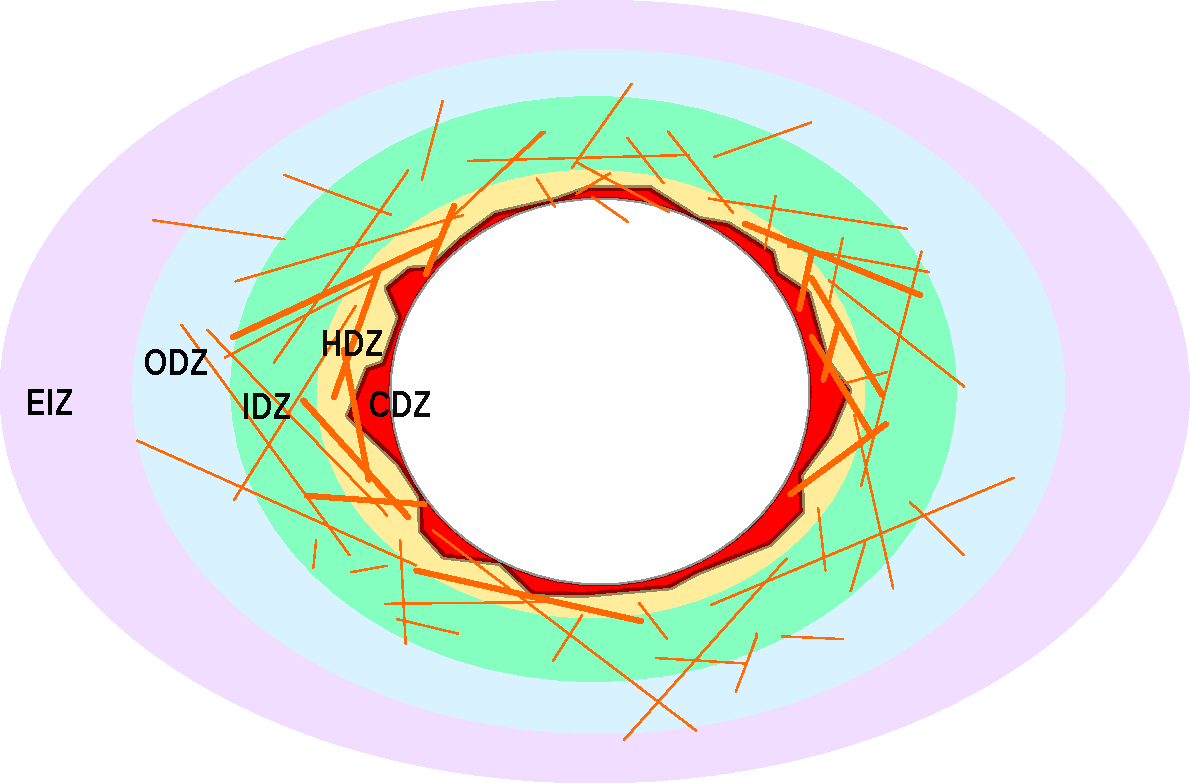
\includegraphics[width=\textwidth]{graphics/EDZ_structure.pdf}
    \caption{Označení zón s kvalitativně odlišnými změnami v~důsledku vzniku díla.}
    \label{fig:edz_zones}
\end{figure}

V projektu nebudeme uvažovat zónu CDZ. V případě použití razícího stroje (TBM -- Tunnel Boring Machine) je rozsah této zóny zanedbatelný, okolo 1~cm. V případě 
ražby střílením je rozsah CDZ významný, až 1~m, ale je prakticky nemožné ho predikovat modelem. Charakterizaci CDZ je případně nutné provést in-situ.
Zbylé zóny vznikají v~důsledku změny okrajové podmínky na stěně díla. Pro jejich vznik jsou klíčové procesy ve dvou různých škálách. V měřítku rozměru 
díla probíhá hydro-mechanický proces redistribuce napětí a~mimo EIZ se jedná o~nevratné plastické změny. Ty však jsou v~případě křehkých hornin
způsobeny nelineárními procesy na mikro puklinách, kde dochází k překonání třecích sil mezi stěnami nebo porušení jejich výplní. 
Změny v~rozevření puklin pak způsobují změny porozity a~hydraulické vodivosti. 

Mikroskopický model a~určení homogenizovaných parametrů EDZ budou diskutovány v~následující kapitole.
V této kapitole se zaměříme na možné makroskopické modely se zahrnutím plasticity a~porušení materiálu.
Nejprve popíšeme scénář a~geometrii úlohy, následně stručně představíme hierarchii modelů se zvyšující se složitostí
a~v~dalších kapitolách pak popíšeme tyto modely podrobněji.

\subsection{Konceptuální model ražby}
Uvažujeme válcovou oblast $\Omega$ sahající do vzdálenosti $R$ od osy vyříznutého úložného vrtu o~poloměru $r$, délku oblasti označme $L$. Orientační rozměry jsou $R\approx 10\,\mathrm{m}$, $r\approx 2\,\mathrm{m}$, $L\approx 1\,\mathrm{m}$. V případě homogenního materiálu lze využít symetrii vzhledem k posunutí podél osy vrtu a~uvažovat výpočet pouze ve 2D řezu. Pro zahrnutí vlivu nehomogenit je nutný plný 3D výpočet. Na této oblasti uvažujeme následující scénář:

\begin{enumerate}
\item {\bf Počáteční stav.} Počáteční tenzor napětí $\sigma_0$, viz kapitola \ref{sec:sigma0}, nulové posunutí, hydrostatický tlak.
                       
\item {\bf Po vyražení.} Na stěně vrtu se změní okrajová podmínka z nulového posunutí na nulovou tečnou sílu
                         a~atmosférický tlak. Vnější okrajová podmínka v dostatečné vzdálenosti předepisuje nulové posunutí, hydrostatický tlak.
                         Je nutné uvažovat nelineární mechanický model a~modely poškození v~blízkosti tunelu. 
                         
% \sy{Myslím, že je zde nezbytné uvažovat následující kombinaci modelů. 1. Na velké geometrii použijeme lineární pružnost a vypočítáme napěťový stav. 2. Na základě výsledků lineární pružnosti sestavíme menší 2D nebo 3D geometrii s detailem tunelu a na této menší geometrii pak aplikujeme vhodný nelineární model,  viz \cite{Blaheta2013a}.}        
% \jb{Rozumím, můj návrh je asi příliš zjednodušující. Je zde také otázka vlivu ostatních chodeb.
% Zatím bych tím nekomplikoval srozumitelnost textu, ale je nutné to uvážit.}

                         
\item {\bf Po zatopení.} Na stěně vrtu se změní okrajová podmínka na hydrostatický tlak, případně tlak bentonitu. Jedná se o~menší změnu, lze tedy uvažovat jednodušší mechanický model. Další vlivy pro jednoduchost neuvažujeme, viz. \ref{sec:micro_EDZ}.
                        
% \sy{Mechanické poškození EDZ může ještě zvýšit šíření tepla od vyhořelého paliva, viz \cite{Blaheta2013a}.}
% \jb{Ano, těch vlivů je více, ale záměrně uvažujeme jen mechanické vlivy.}
\end{enumerate}

Výsledkem makroskopického modelu bude rozložení napětí a~deformace po ražbě a~po zatopení. Pro výpočet budou použity 
parametry konstitutivních vztahů určené pomocí mikro modelu, viz kapitola \ref{sec:micro_EDZ}. 

Vlivem přítomnosti podzemní vody a~relativně malé hydraulické vodivosti krystalických hornin dochází k redistribuci napětí 
postupně v~horizontu asi jednoho roku. To je z hlediska stanovení vlastností EDZ po zatopení zanedbatelné a~je tedy možné uvažovat 
pouze stacionární hydro-mechanickou úlohu. Nicméně plný hydro-mechanický model relaxace napětí lze použít pro stanovení vlastností EDZ (viz kapitola \ref{sec:experiment}).







\subsection{Přehled kontinuálních modelů} 

Pro výpočet poškození hornin je vhodné uvažovat hierarchii modelů se zvětšující se složitostí, viz \cite{Blaheta2013a}, a~také různou potřebou vstupních parametrů:
\begin{enumerate}[(i)]
	\item \label{mod_elast} {\bf Elastický model.} Elastický výpočet napětí a~deformací a~následně indikace, kde dochází k porušení materiálu podle vhodného pevnostního kritéria.
	\item \label{mod_plast} {\bf Plastický model.} Výpočet napětí a~deformací za předpokladu, že nemůže dojít ke stavům za mezí platnosti vhodného pevnostního kritéria (plastické modely). Lze uvažovat procesy s~postupným zatěžováním a~monotónní odezvou (deformační teorie plasticity) i modely se zatěžováním a~odlehčováním a~trvalými (plastickými) deformacemi,
	\item \label{mod_damage} {\bf CDM -- Continuum Damage Mechanics}. Výpočet napětí a~deformací za předpokladu, že nemůže dojít ke stavům za mezí platnosti vhodného pevnostního kritéria a~zároveň dochází k oslabení (porušování --  damage) materiálu. V případě samotné Damage Mechanics se neuvažují nevratné deformace.
	\item \label{mod_irev_cdm} {\bf Kombinované modely.} V praxi existuje řada kombinací výše uvedených modelů. Jednak lze uvažovat kombinaci plasticity a~Damage Mechanics, která uvažuje jak oslabení, tak i trvalé deformace. Existuje však také mnoho ad-hoc přístupů, které uvažují postupné oslabování materiálových konstant, viz např. \cite{Perras2016}, \cite{Carranza-Torres1999}.
\end{enumerate}
U modelů \eqref{mod_elast} a~\eqref{mod_plast} máme většinou řadu informací o~existenci a~jednoznačnosti
řešení, o~stabilitě, tedy spojité závislosti řešení na vstupních datech, o~chybě vznikající  při  diskretizaci  úloh  atd.  Složitější je porozumění  modelům CDM, pro které existuje závislost diskretizovaných  modelů na  síti, nejednoznačnost řešení  apod. Proto jsou navrženy CDM modely s~regularizací nebo s~nelokální definicí deformací a~napětí. 




\subsection{Elastický model}

Základním modelem pro výpočet napětí a~deformací je lineární elasticita s~tenzorem malých deformací a~Cauchyovým tenzorem napětí, která je popsána trojicí veličin: posunutí $\vc u$, deformace $\eps$ a~napětí $\sigma$, a~jejich vzájemnými vztahy, které platí ve výpočetní oblasti $\Omega$:
\begin{align*}
	- \div(\sigma) &= \vc f &\mbox{v} \ \Omega, \\
	\sigma &= \tn C : \eps + \sigma_0 + p\tn I  &\mbox{v} \ \Omega, \\
	\eps(\vc u) &= (\nabla \vc u + (\nabla \vc u)^\T &\mbox{v} \ \Omega.
\end{align*}
Výše, $\vc f$ vyjadřuje hustotu objemových sil (dále neuvažujeme), $\sigma_0$ je počáteční napětí a $p$ pórový tlak vody. 
Klíčový konstitutivní parametr elastický tenzor pružnosti $\tn C$ má pro izotropní materiály tvar:
\[
    \tn C_{ijkl} = 2\mu\delta_{il}\delta_{jk}+\lambda\delta_{lk}\delta_{ij}  
\]
kde Lamého parametry 
\[
  \lambda = \frac{E\nu}{(1+\nu)(1-2\nu)},\quad \mu=\frac{E}{2(1+\nu)}
\]
 jsou dány Youngovým modulem $E$ $[Pa]$ a Poissonovým číslem $\nu$ $[-]$.



Dále na hranici $\partial \Omega$ musíme zadat vhodné okrajové podmínky. 

V uvedené formulaci jsou kompresní deformace a~normálová napětí v~tlaku záporné (mechanická konvence). 
Hlavní napětí (vlastní čísla tenzoru $\sigma$) pak označíme $\sigma_3 \geq \sigma_2 \geq \sigma_1$.
Pro popis pevnostních veličin se ale v~geotechnice užívá opačná konvence, kdy normálová napětí v~tlaku jsou kladná (geomechanická konvence).
Potom budeme uvažovat hlavní napětí $\sigma_3 \leq \sigma_2 \leq \sigma_1$, kde $\sigma_1$ je největší hlavní napětí, které je obvykle kladné v~tlaku.


\subsubsection{Pevnostní kritéria}
Pevnostní kritéria vychází z vypočteného napětí, případně deformace. Přípustné stavy je možné popsat nerovností
$$
	F_s = F_s(\sigma, \varepsilon) \leq 0.
$$
Kritérii často používanými v~mechanice hornin jsou Mohrovo-Coulombovo a Hoekovo-Brownovo kritérium, viz např. 
\cite{Desai1984}, \cite{Goel2011}, \cite{Zang2010} a~\cite{Brady2006}. Tato kritéria nyní popíšeme za předpokladu izotropní horniny.
\begin{itemize}
	\item Mohrovo-Coulombovo kritérium
		$$
			F (\sigma, x) = |\tau| - (c + \sigma_n \mbox{tg} (\phi)) ,
		$$
		kde $\tau$ a $\sigma_n$ je smykové a normálové napětí působící na libovolnou plochu procházející bodem x, $c$ je koheze a~$\phi$ je úhel vnitřního tření.
	\item Mohrovo-Coulombovo kritérium lze také vyjádřit pomocí hlavních napětí. Kritické napětí se týká plochy, která je rovnoběžná se směrem prostředního hlavního napětí. Pokud její polohu vyjádříme úhlem $\beta$ mezi normálou a~směrem $\sigma_1$, potom na ni budou působit napětí
		$$
			\sigma_n = \frac{1}{2}(\sigma_1 + \sigma_3 ) + \frac{1}{2}(\sigma_1 - \sigma_3 )\cos 2 \beta, \quad \tau = \frac{1}{2}(\sigma_1 - \sigma_3 ) \sin 2 \beta.
		$$
		Kritický poměr pak nastane pro $\beta =  \frac{\pi}{4} + \frac{\varphi}{2}$. Pro tento úhel dostaneme
		$$
			F(\sigma,x) = (\sigma_1 - \sigma_3 ) - \frac{2c\,\cos \phi}{1-\sin \phi} - \frac{2\sin \phi}{1-\sin \phi} \sigma_3 .
		$$
		Kritérium lze také vyjádřit vztahem
		$$
			F(\sigma, x) = (\sigma_1 - \sigma_3) - (q_{cmass} + A\sigma_3) \leq 0
		$$
		kde $q_{cmass}$ je jednoosá pevnost v~tlaku (UCS) pro masiv,
		$$
		q_{cmass} = \sigma_c = \frac{2c \cos \phi}{1-\sin \phi}, \quad 
		A = \frac{2 \sin \phi}{1-\sin \phi}.
		$$ 
		UCS lze interpretovat jako Uniaxial Compressive Strength (značí se obvykle $\sigma_c$), nebo Unconfined Compressive Strength ($q_c$). Lze také využít pevnost v~tahu (tensile strength $\sigma_t$),
		$$
             \sigma_t = \frac{2c \cos \phi}{1+ \sin \phi}.
		$$
		Další možností je vyjádření kritéria nikoli pomocí hlavních napětí, ale pomocí invariantů napětí. Viz např. \cite{Desai1984}.
	\item Mohrovo-Coulombovo kritérium bývá také doplněno podmínkou žádného či částečného nepřipuštění tahových napětí (tension cut-off).
	\item Hoekovo-Brownovo kritérium je možno považovat za zobecnění Mohrova-Coulombova kritéria. Toto zobecnění bylo určeno empiricky a~zohledňuje kvalitu hornin s~uvažováním jednoosé pevnosti v~tlaku (UCS) pro neporušenou horninu $q_c$ na jedné straně, ale parametry charakterizující kvalitu (porušenost) hornin, na straně druhé. 					Kritérium má tvar
		$$
			F(\sigma,x)=(\sigma_1 - \sigma_3 ) - q_c \left[m_b \frac{\sigma_3}{q_c} + s \right]^a ,
		$$
		kde $q_{c}$ jednoosá pevnost v~tlaku neporušených kusů horniny, $m_b$ je nelineární parametr závisející na typu horniny, $a$ je parametr rozpukání horniny.
\end{itemize}

\subsection{Plastické modely}
\alert{Perfektně} plastický model je ve tvaru
\begin{table}[ht]
	\centering
	\begin{tabular}{ll}
		\hline
		rozklad tenzoru deformace & $\varepsilon = \varepsilon^e + \varepsilon^p$\\
		Cauchyho napětí & $\sigma = C : \varepsilon^e$\\
		\alert{plastické kritérium} & \alert{$f_p(\sigma)\leq0$}\\
		plastický potenciál & $g_p,\;\;$ daný vztahem: $\partial g_p/\partial \sigma = \partial f_p/\partial \sigma$  \\
		plastické tečení & \alert{$\dot{\varepsilon}^p = \dot{\gamma}(\partial g_p/\partial \sigma), \dot\gamma \geq 0$,}\\
		podmínka duality & $\dot{\gamma} f_p =0$\\
		\hline
	\end{tabular}
\end{table}

\begin{itemize}
	\item V případě Mohrovy-Coulombovy plasticity máme
	\begin{eqnarray*}
		f_p(\sigma) &=& \frac{1}{2} (\sigma_1 - \sigma_3) + \frac{1}{2} (\sigma_1 + \sigma_3)\sin \phi - c \cos \phi, \\
		g_p(\sigma) &=& \frac{1}{2} (\sigma_1 - \sigma_3) + \frac{1}{2} (\sigma_1 + \sigma_3)\sin \psi,
	\end{eqnarray*}
	\alert{kde $\psi$ je úhel dilatace (dilation angle), viz \cite{Neto2011}. Poznamenejme, že pro $\phi = \psi$ platí $\partial g_p/\partial \sigma = \partial f_p/\partial \sigma$, a~tedy se jedná o~asociovaný model. Dále, plastické kritérium $f_p(\sigma)\leq0$ je ekvivalentní s~výše uvedeným kritériem, což odvodíme přenásobením funkce
	$F(\sigma, x) = (\sigma_1 - \sigma_3) - \frac{2c\cos \phi}{1-\sin \phi} - \frac{2\sin \phi}{1-\sin \phi} \sigma_3$ výrazem $\frac{1}{2}(1 - \sin \phi)$.}
	\item Místo Mohrovy-Coulombovy plasticity lze také použít Druckerův-Pragerův model, jehož popis i vztah k parametrům Mohrovy-Coulombovy plasticity lze najít v~\cite{Neto2011}. 
	\item Plasticita vycházející z Hoekova-Brownova kritéria je málo obvyklá, ale možná. Viz např. \cite{Carranza-Torres1999}.
\end{itemize}


\subsection{Modely s poškozením}
Samotné modely plasticity neuvažují oslabení materiálu při křehkém porušení. K tomu účelu můžeme zavést parametr oslabení (damage parameter) $\omega\in[0,1]$, kde $\omega = 0$ odpovídá neporušenému materiálu a~$\omega = 1$ znamená zcela porušený materiál.
Nejjednodušší kombinace elasticity a~porušení by potom využívala vztahy
\begin{table}[h!]
	\centering
	\begin{tabular}{ll}
		\hline
		zobecněný Hookův zákon & $\sigma = (1-\omega)C : \varepsilon$\\
		vývoj porušení & $\omega = g(\kappa), \dot{\kappa} \geq 0, \kappa(0) = \overline{\varepsilon}_0$\\
		funkce porušení & $f_d(\varepsilon,\kappa)=\overline{\varepsilon}(\varepsilon)-\kappa$\\
		podmínka přípustnosti & $f_d(\varepsilon,\kappa)\leq 0$ \\
		podmínku duality & $\dot{\kappa} f_d =0$\\
		\hline
	\end{tabular}
\end{table}

Výše $\overline{\varepsilon}(\varepsilon)$ představuje ekvivalentní tahovou deformaci
$$
	\overline{\varepsilon}(\varepsilon) = (\langle\varepsilon_1\rangle^2+\langle\varepsilon_2\rangle^2+\langle\varepsilon_3\rangle^2)^{1/2},
$$
kde $\langle\varepsilon_i\rangle$ značí absolutní hodnotu tahových hlavních deformací, deformace
v~tlaku se neuvažují. Všimněme si souvislosti s~pevnostními kritérii využívajícími deformace, přehled lze nalézt v~\cite{kwasniewski_strain_based_2010}.
Parametr porušení se vyvíjí v~závislosti na zavedené ekvivalentní tahové deformaci. Funkci $g$ můžeme volit exponenciálně s~adaptací na diskretizační parametr.

Modelování porušení CDM je poměrně složité, viz např. \cite{Lemaitre1992}, \cite{Neto2011}, \cite{GJ06}, \cite{UH15}. Proto pouze zmíníme některé složitější podrobnosti:
\begin{itemize}
	\item porušení nemusí být izotropní a~může být také odlišné pro namáhání v~tlaku a~tahu,
	\item v~reálných případech se při porušení objevují trvalé deformace, takže
	použijeme opět dělení deformací $\varepsilon=\varepsilon^e + \varepsilon^p$, $\overline{\sigma} = C : \varepsilon^e$, $\sigma = (1-\omega)\overline{\sigma} = C : \varepsilon^e$. Navíc propojíme růst poškození s~přírůstkem plastické deformace, $\dot{\kappa} = \|\dot{\varepsilon}^p\|^2 = \dot{\varepsilon}^p : \dot{\varepsilon}^p$.
	\item modely poškození je nutné stabilizovat pro zamezení závislosti na diskretizaci.
\end{itemize}


\subsection{Nejistoty v parametrech mechaniky}

\subsubsection{Počáteční napětí}
\label{sec:sigma0}
Počáteční napětí výrazně ovlivňuje výsledné napěťové pole a~tím i charakter EDZ.
V horninovém masívu s~elastickým chováním a~s~Poissonovou konstantou $\nu$, v~hloubce $h$ a~s~průměrnou hustotou nadložních hornin $\rho_{r}$ a~v~případě,
že na horniny nepůsobí jiné vlivy než váha hornin, je počáteční napětí $\sigma_0$
popsáno hlavními napětími ve směrech souřadného systému $(\sigma_x, \sigma_y, \sigma_z)$ určenými vztahem
\begin{equation}
	\sigma_z = h\,\rho_{r}\, g, \quad \sigma_x = \sigma_y = \frac{\nu}{1-\nu} \sigma_z,
\end{equation}
přičemž $g$ je gravitační konstanta. Pro hloubku 500 m a $\nu = 1/4$ uvedené vyjádření dává hodnoty
$$
	\sigma_z = 13.5, \sigma_x = \sigma_y = 4.05\quad [\mathrm{MPa}].
$$
Reálná počáteční napětí však mohou mít převažující horizontální složky a~obecné vlastní vektory (nerovnoběžné se souřadným systémem). Například napětí měřené v~hloubce 420 m v~Underground Research Laboratory (URL) blízko Lac du Bonnet, Manitoba, Kanada, dosahuje hodnot
$$
	\sigma_3 = 11, \sigma_2 = 45, \sigma_1 = 60\quad [\mathrm{MPa}]
$$
viz \cite{Rutqvist2009}. V tomto případě musíme počítat i se smykovými napětími. Počáteční napětí může být velmi proměnné i~v~rámci jedné lokality, zvláště pokud je navíc ovlivněna více podzemními díly, viz příklad laboratoře GRIMSEL ve Švýcarsku, viz \cite{Krietsch2019},
\cite{Stas2016}, \cite{Rutqvist2004}. Pro studium EDZ je proto vhodné uvažovat výpočty pro různé hodnoty počátečního napětí.
Poznamenejme  ještě, že počáteční napětí $\sigma_0$ může být určeno přímým měřením nebo měřením poloh referenčních bodů 
a výpočtem pomocí inverzní analýzy, viz \cite{Malik2021}, \cite{Soucek2017}.


Počáteční napětí je klíčový parametr a je nutné jej uvažovat jako náhodnou veličinu se zahrnutím 
chyby měření (např. v \cite{Herget1973} okolo 10\%). V rámci oblasti $\Omega$ s rozměry do 10m není patrně nutné uvažovat prostorovou 
závislost $\sigma_0$ a to ani změnu s hloubkou (pro hloubku okolo 500m bude vliv hloubky do 2\% což je pod úrovní chyby měření).


\subsubsection{Konstitutivní vztahy}
Za předpokladu isotropní horniny, bude uvažován modul pružnosti $E$  jako korelované náhodné pole 
a Poissonovo číslo $\nu$ jako (homogenní) náhodná veličina. Generování korelovaných polí pro případ 
anisotropní horniny je popsán v \cite{Tang2018}.

Pro plastické modely je třeba zadat další parametry, např. Hoek-Brownovo kritérium obsahuje parametry:
$\sigma_c$, $m$, $s$, $a$. Jednoosá pevnost v tlaku $\sigma_c$ je patrně ovlivněna nehomogenitami horniny a bude proto vhodné 
ji modelovat jako  korelované náhodné pole. Ostatní parametry charakterizují typ a porušení horniny. Lze uvažovat jako pevné konstanty
a volit dle prací: \cite{Martin1999}, \cite{Hajiabdolmajid2002}, \cite{Hoek2002} s ohledem na konkrétní charakterizaci horniny.

V případě použití modelů s poškozením bude nutné specifikovat vhodné konstitutivní vztahy další rešerší.


Při použití víceškálového přístupu, viz. sekce \ref{sec:mikroskala}, lze uvažovat parametry jako skalární náhodné veličiny a
prostorovou nehomogenitu popsat pouze náhodnou sítí puklin.



\section{Efektivní vlastnosti EDZ}
\label{sec:micro_EDZ}
Změny napětí způsobené ražbou resp. zatopením díla vedou ke změnám klíčových parametrů transportního modelu:
permeability $\kappa$ a~porozity $\theta$. V menší míře mohou být ovlivněny i parametry $d_m$, $\alpha_L$, $\alpha_T$.

Kromě mechanických změn mohou mít na hodnotu těchto parametrů vliv i~další procesy zejména změny teploty v~důsledku radioaktivního rozpadu, viz. \cite{Blaheta2013a}, 
a~chemické procesy vedoucí k hojení mikrotrhlin. Jakkoliv mohu být významné, nebudou pro zachování jednoduchosti tyto procesy uvažovány.
Stejně tak nebude uvažována žádná metoda sanace EDZ (např. různé druhy tlakové penetrace).

V této kapitole představíme možné modely závislosti parametrů transportu na napětí a~deformaci.
Nejprve v~sekci \ref{sec:empiricke} uvedeme některé publikované empirické vztahy pro vodivost a~porozitu.
Tyto empirické vztahy stejně jako konstitutivní vztahy mechanických modelů z kapitoly \ref{sec:model_EDZ} 
obsahují volné parametry, které lze sice určit pomocí laboratorních měření, avšak toto měření je provedeno na intaktních vzorcích,
a proto není přímo přenositelné na větší škály s~výskytem větších poruch. Jednou možností, jak toto omezení obejít, je
použití víceškálového přístupu popsaného v~sekci  \ref{sec:mikroskala}.


\subsection{Závislost na mechanice}
\label{sec:empiricke}

Pro porézní médium složené z částic (písek, štěrk) má poměrně širokou platnost vztah Kožený-Carman \cite{Carman1956}, \cite{Carrier2003}:
\begin{equation}
  \label{eq:Kozeny}
  \kappa = \frac{1}{C_{KC}a^2}\frac{e^3}{1+e},
\end{equation}
kde $C_{KC}$ $[-]$ je empirická konstanta, $a$  $[\mathrm{m}^{-1}]$ je specifický povrch částic na jednotkový objem a~$e$ $[-]$ je  \uv{void ratio} --
poměr volného objemu ku objemu částic. Ten lze zapsat pomocí porozity:
\[
   e = \frac{\theta}{1 - \theta}.
\]
Změny porozity $\theta$ vůči počáteční porozitě $\theta_0$ jsou dány stopou tenzoru deformace $\eps$:
\begin{equation}
   \label{eq:porozity_deformation}
   \theta = \frac{\theta_0 + \tr(\epsilon)}{1 + \tr(\epsilon)}.
\end{equation}
Tímto dostáváme jednoduchý vztah pro závislost permeability a~porozity na deformaci. Pro EDZ je tento přístup nedostatečný kvůli anizotropii
puklin a~nelineární mechanice, t.j.  porušení vztahu \eqref{eq:porozity_deformation}.

Pro systém paralelních rovinných puklin s~jednotkovou normálou $\vc n$, rozevřením $d$ $[\mathrm{m}]$ a~vzdáleností $D$ $[\mathrm{m}]$
byl odvozen kubický zákon \cite{Snow1969}:
\[
 \kappa = \frac{d^3}{12 D} (\tn I - \vc n \otimes \vc n).
\]

Základním článkem studujícím změny vodivosti v~EDZ je \cite{Kelsall1984}. Přímou aplikací normálového napětí
na jednu puklinu a~použitím kubického zákona je odvozen empirický vztah pro permeabilitu jedné pukliny:
\[
  \kappa = \kappa_0 \Big[A (\frac{\sigma_e}{\eta})^t+1\Big]^{-3},
\]
kde $\kappa_0$ je počáteční permeabilita, $\sigma_e$ je normálové napětí a~$A$, $\eta$, $t$ jsou empirické parametry.
V porovnání s~uvedeným měřením je však dosaženo pouze hrubé shody. Celkově je pozorováno zvýšení vodivosti v~EDZ o~jeden až dva řády jen díky změnám napětí.
Článek dále studuje i vliv ražby na hydraulickou vodivost se závěrem, že vliv ražby převažuje zhruba do 30~cm od stěny díla. 


V přehledovém článku \cite{Rutqvist2003} věnovanému hydro-mechanickým modelům pro rozpukané horniny
je pro neporušenou horninu citován vztah Kožený-Carman a~několik jednodušších empirických aproximací, např.
exponenciální model:
\[
  \kappa=\kappa_0 \exp(-a_1 P)
\]
a 
mocninný model:
\[
  \kappa=\kappa_0 P^{-a_2},
\]
kde $a_1$ a $a_2$ jsou empirické konstanty a~$P=P_c - p$ je efektivní tlak pro kompresní tlak horniny $P_c$ a~proti působící tlak vody $p$.
Pro vodivost puklin (transmisivitu) je základem kubický zákon, kde je jednak použito různě chápané \uv{hydraulické} rozevření pukliny $d_h$ 
a dále je prezentována celá řada vztahů pro závislost změny reálného rozevření $d$ na normálovém a~smykovém napětí. Například logaritmický vztah 
podle \cite{Kohl1995} pro změnu rozevření pukliny
\[
   d - d_0 = - C \ln \frac{\sigma_n}{\sigma_0},
\]
kde $d_0$ a $\sigma_0$ jsou počáteční rozevření a~počáteční normálové napětí. 

Pro hydro-mechanický model odezvy na ražbu tunelu TSX (URL, Kanada), \cite{Rutqvist2009}, viz též kapitola \ref{sec:experiment}, byl použit vztah:

$$
	\kappa = \kappa_0 \mbox{exp}(\beta e_d),
$$
kde $\kappa_0$ je permeabilita neporušeného masivu, $\beta$ je empirický parametr, $e_d$ je ekvivalentní
deviatorická deformace,
$$
	e_d = \frac{2}{\sqrt{6}}[(\varepsilon_1 - \varepsilon_2)^2 + (\varepsilon_2 - \varepsilon_3)^2 + (\varepsilon_3 - \varepsilon_2)^2]^{1/2},
$$
kde $\varepsilon_1$, $\varepsilon_2$ a~$\varepsilon_3$ jsou hlavní deformace.


Tento ani předchozí citované vztahy nedávají možnost kombinace smykového a~normálového napětí a~nepopisují 
nárůst vodivosti při velkých napětích. Tento efekt je popsán v~\cite{Souley2001}, kde je též navržen model poškození (CDM)
a~nárůst vodivosti je vysvětlen propojením zvětšujících se mikro trhlin do souvislé vodivé sítě.
Je zde ale uvažována pouze izotropní vodivost. Tento konceptuální model již je blízko explicitnímu popisu dějů na puklinách 
pomocí mikro škálového modelu.

Další práce a~alternativní přístupy lze nalézt v~přehledovém článku \cite{Shahbazi2020a}. 




\subsection{Víceškálový přístup}
\label{sec:mikroskala}
Konstitutivní vztahy mechanických modelů a~vztahy závislosti permeability na napětí či deformaci vyžadují určení 
několika volných parametrů. Tyto parametry není možné určit laboratorním měřením na vzorcích (o rozměru cca 0.1~m), 
jelikož reálné kontinuum ve větší škále (cca 10~m) obsahuje systém větších puklin, které laboratorní měření nezachytí. 
Stanovení volných parametrů z měření in-situ je nákladné a~náchylné na systematické chyby kvůli nemožnosti 
více nezávislých pozorování. 


Navrhujeme proto použít následující víceškálový přístup:
\begin{itemize}
 \item Předpokládáme měření (deformace a~hydraulické vodivosti při zatížení) na laboratorních vzorcích o~rozměru $l=0.1\,\unit{m}$ obsahujících pukliny do velikosti $r=1\,\unit{cm}$.
 \item Uvažujeme oblast odpovídající laboratorním vzorkům (krychle o~straně $l$) se sítí náhodných puklin menších než $r$.
 \item Na oblasti řešíme úlohu s~elastickým kontinuem a~diskrétními puklinami s~explicitním popisem jejich kontaktů, tření a~rozevírání.
       Plasticita a~poškození by měly být postihnuty pomocí procesů na puklinách. Fitujeme parametry $P_f$ puklin (např. model tření nebo závislost vodivosti na rozevření) a~parametry kontinua. 
 \item Na oblasti bez diskrétních puklin řešíme stejnou úlohu s~plastickým modelem a~fitujeme parametry $P_c$ konstitutivních vztahů kontinua.
 \item V makro modelu uvažujeme diskrétní pukliny velikosti větší než $r$ a~použijeme nafitované parametry $P_f$ pro kontinuum použijeme parametry $P_c$.
\end{itemize}
Jelikož je systém puklin statisticky soběpodobný ve velkém rozsahu škál, lze uvažovat jeden statistický model puklin pro všechny škály modelů.
Parametry statistického modelu pak lze poměrně levně určit mapováním puklin na stěnách díla a~z~karotáží, viz \cite{Bonnet2001}.
Zároveň předpokládáme, že parametry vztahů pro vlastnosti puklin jsou již nezávislé na měřítku, 
jelikož velikost puklin v~nich již vystupuje explicitně. 

Víceškálový přístup v~různých podobách byl již využit v~řadě prací zabývajících se vztahem mezi mechanikou a~vodivosti. 
Motivující pro nás byla práce \cite{Min2004a}, kde je demonstrováno, jak poměrně jednoduchý model puklin
s~kontakty třením a~rozevíráním při tečném posunutí
dokáže postihnout růst vodivosti při větším napětí, jak je popsáno, ale vysvětleno jinak v~\cite{Souley2001}.
Navíc je zde demonstrována dobrá shoda s~kontinuálním modelem využívajícím empirických vztahů pro popis vodivosti kontinua v~závislosti na napětí.

Další motivací je popis mechanického modelu s~poškozením \cite{Shao2005}, kde jsou homogenizované konstitutivní vztahy ekvivalentního kontinua
odvozeny pro síť mikro puklin s~daným rozdělením orientací. Pro analytický výpočet ekvivalentního tenzoru permeability je pak využit postup superpozice tenzorů 
pro různé orientace puklin, viz \cite{Oda1986a}.

Nakonec lze zmínit novější práci, \cite{Rutqvist2013}, kde je popsán hydro-mechanický model s~víceškálovým přístupem. Je vygenerována síť (jemných) 
puklin a~pro podoblasti odpovídající elementům makro úlohy jsou stanoveny efektivní parametry kontinua nikoliv pomocí řešení  úlohy na DFN síti, 
ale pomocí numerické superpozice tenzorů, viz \cite{Oda1986a}. Celý postup je pak validován vůči výpočtu na jemné DFN síti.



% TODO:
% - otázka zda je difúze zanedbatelná při malých rychlostech
% - zjistit řádově rychlosti na úrovni úložiště
% - pro začátek bychom difúzi zanedbali
% 
% - klíčový parametr tenzor počátečního napětí
%   lze měřit a~lze získat 
% 
% - výpočet 
% - tlak bentonitu 2,5 az 5 MPa, to je zhruba srovnatelne s~hg tlakem v 500m cca 5MPa
% - Grimsel v zule + teplo, pomala saturace, nebyla saturace ani po 18letech
% - 





% \subsection{Rešerše - přehled souvisejících článků}
% {\bf \cite{Shahbazi2020a}}\\
% Přehledový článek o~různých analytických a~numerických modelech 
% pro prdikci hydraulické vodivosti rozpukaného prostředí i na základě mechaniky. Z numerických přístupů 
% jsou použity převážně DFN (discrete fracture networks) a~DEM (distinct element method). 
% TODO: projiít odkazy, hledání multiscale přístupu, jednoduchý model pro jemnou škálu s~puklinami, 
% efektivní parametry pro makro škálu
% 
% \noindent{\bf \cite{Blaheta2013}}\\
% TH model pilíře v laboratoři \"Asp\"o se zahrnutím plasticity a~modelů poškození. 
% Kalibrace na některé měřené veličiny.
% 
% 
% 
% \noindent{\bf \cite{Perras2016}}\\
% Použití DISL - damage initiatin and spalling pro predikci hloubky jednotlivých částí EDZ,
% porovnání numerických modelů a~empirických dat, fitování empirického vztahu pro relativní hloubku 
% ($r/R$) v závislosti na maximálním tečným napětím na stěně normalizovaném na CI (crack initiation napětí)
% ,$\sigma_{max} / \sigma_{CI}$. To je nelineární rozšíření vztahu navrženého v
% \cite{Martin1999} a~\cite{Diederichs2007}). 
% DISL je založen na Hoek-Brownově kritériu.
% 
% \noindent{\bf \cite{Martin1999}}\\
% Analýza hloubky poškození v závislosti na napětí a~tvaru tunelu, krystalinika, založeno na Hoek-Brown.
% 
% \noindent{\bf \cite{Dreuzy2012}}\\
% Porovnání DFN s~konstantní vodivostí puklin vs. puklin s~heterogenní vodivostí (Gaussian distribution, power-law like correlation). Analýza vlivu celkovou vodivost sítě. Pro heterogenní případ pozorováno převážně snížení celkové vodivosti (faktorem 2 - 6). \todo{podrobnější čtení}
% 
% 
% 
% \noindent{\bf \cite{Souley2001}}\\
% Model poškození a~model změny permeability v závislosti na mechanice, vychází z konceptu paralelních puklin \cite{Snow1965}. Zaměřeno na krystalické horniny, neuvažuje namáhání v tahu.  Implementováno v SW FLAC3D (použit v projektu "Hluboké horizonty").
% 
% \noindent{\bf \cite{Rutqvist2003}}\\
% Přehled HM modelů pro rozpukanou horninu s~různými konstitutivními 
% vztahy pro explicitní popis vlastností puklin v závislosti ne tečném a~normálovém napětí. 
% Příklady aplikací a~porovnání s~měřeními.
% Vztah mezi permeabilitou a~"confining pressure" 
% (pokles vodivosti s~hloubkou. Jsou diskutovány vztahy mezi napětím resp. 
% porozitou a~permeabilitou. Matematický popis jevů na puklinách. Rozdíl mezi "apparent aperture" 
% a~"real apperture". 
% 
% \noindent{\bf \cite{Rutqvist2009}}\\
% TSX experiment, calibration of plasticity model and permeability dependance on the strain through the HM-model of stress relaxation
% 
% 
% 
% {\bf \cite{Kelsall1984}}:\\
% Základní článek zabývající se otázkou změny hydrulické vodivosti v EDZ. 
% Odvozeno analytické řešení pro rozložení napětí v okolí ideální kruhové chodby. 
% Změny v hydraulické vodivosti jsou dále odvozeny na základě kubického zákona. 
% Na základě tohoto modelu predikují zvýšení vodivosti o~jeden až dva řády pouze vlivem změny napětí. Změna alespoň o~jeden řád nejvýše do vzdálenosti dvou průměrů od stěny chodby. Ražba střílením může dále zvýšit hydraulickou vodivost, avšak jen v blízkosti (cca. 0,3 m) stěny chodby.
% 
% 
% {\bf \cite{Lisjak2014}}\\
% Modelování vzniku puklin v EDZ pomocí \uv{hybrid finite discrete elements method},
% přehled jiných numerických přístupů. 
% 
% {\bf  \cite{Barton1985}}\\
% Measurement of fracture apperture and "real" apperture used in models.
% 
% {\bf \cite{Shao2005}}\\
% Mechanické vlastnosti a~permeabilita křehkých hornin, vztahy odvozené na základě sítě mikropuklin, zahrnut vliv propojenosti, porovnání s~laboratorními experimenty. Asi nejblíže našemu záměru, netriviální formulace mechaniky pomocí mechanické entalpie a~nejasné odvození.


\section{Metody měření parametrů EDZ}
\label{sec:parameters}

Při využití navrženého víceúrovňového přístupu lze provést výpočty i pouze na základě laboratorních měření avšak měření in-situ budou
nutná jednak pro validaci celého přístupu i konkrétního modelu a dále pro přesnější celkové nastavení modelu. Tato kapitola představuje
rešerši existujících metod pro identifikaci vlastností EDZ, zejména: 

\begin{itemize}
 \item {\bf puklinová síť} - četnosti, orientace, velikost a rozevření puklin
 \item {\bf mechanika} - modul pružnosti, poissonovo číslo, anisotropie, parametry plastických modelů
 \item {\bf proudění} - permeabilita a porozita pro jednotlivé pukliny, pro EDZ, pro intaktní horninu
 \item {\bf transport} - tortuozita, příčná a podélná disperzivita
\end{itemize}

Rešerše vychází zejména ze rešeršních prací \cite{Vavro2016} a \cite{Lanyon2011} a jejich referencí. 
Pozornosti také zasluhuje \cite{Chandler2002} kde je mimo jiné prezentována řada metod aplikovaných na EDZ v rámci experimentu TSX.



\subsection{Geologická charakterizace, mapování puklin}
\label{sec:mapovani_puklin}
\subsubsection{Mapování na vrtech}
Před ražbou i po ní je možné provádět charakterizaci hornin a mapování puklin pomocí vrtů. 
Při získání jader lze charakterizovat porušenost horniny pomocí vhodného indexu (např. RMR nebo GSI), 
které lze využít k určení některých parametrů plastických modelů \cite{Hoek2002}. 
Pro mapování puklin je vhodnější akustická (HiRAT) nebo optická (OPTV) karotáž. Získané snímky je možno 
zpracovat strojově pro identifikaci puklin, \cite{Tammisto2002}, což může odstranit subjektivní vliv při manuálním zpracování.
Mapování na vrtech považujeme za středně náročné jelikož vrt lze použít k získání většího množství dat 
a samotné mapování je poměrně nenáročné.

\subsubsection{Mapování na stěnách díla}
Po vyražení díla je možno províst geologickou charakterizaci včetně mapování puklin podobně jako pro vrty, 
zde je podstatná metodika mapování, \cite{Bossart2002},  pro minimalizaci subjektivních vlivů. 
V případ ražby odstřelem je možné využít laserové 3d skenování pro kvantitativní hodnocení 
nadvýlomů a dalších charakteristik kvality ražby \cite{Hudson2009a}. 
Pro získání parametrů statistického modelu (sekce \ref{sec:dfn}) je nutno zohlednit výběrový efekt 
mapovaných vrtů a mapovacích technik, viz. \cite{Zetterlund2012}, \cite{Torabi2011}. 
Mapování na stěnách díla je technicky nenáročné, ale vyžaduje pečlivou metodiku a může být časově náročné.

\subsubsection{Injektáž pryskyřicemi}
Pro lepší identifikaci puklin včetně jejich konektivity je možno do úzkého vrtu pod tlakem aplikovat 
pryskyřici s přídavkem fluoresceinu. Po vytvrdnutí (cca 3 týdny) je vzorek odvrtán širším průměrem a jádro je pozorováno pod UV světlem.
Pryskyřice zajistí soudržnost jádra a flourescein umožní velmi dobrou vizualizaci puklinové sítě, \cite{Bossart2002}, \cite{Lanyon2011}
Metoda je poměrně náročná technicky i časově.


\subsection{Geofyzikální měření}
Geofyzikální měření jsou atraktivní kvůli neinvazivní charakterizaci horniny
avšak jsou z principu metodami nepřímými, kdy výsledná (prostorová) charakterizace
horniny je výsledkem inverzní úlohy. Jsou poměrně levné, avšak nelze je obvykle použít k identifikaci 
hodnot parametrů horniny, spíše k popisu heterogenit a rozhraní. Měření je obvykle možno provádět na stěnách díla nebo 
vrtu, nebo mezi více vrty (tomografie).

\subsubsection{Seismické a akustické metody}
Existuje množství metod využívající šíření mechanického vlnění (zvuku) v hornině. Zde popíšeme čtyři metody použité v rámci experimentu TSX, URL, Kanada,  \cite{Chandler2002}.

{\bf Refrakční seismika} umožňuje detekovat rozhraní mezi porušenou vrstvou s nižší vlnovou rychlostí a neporušenou vrstvou s vyšší vlnovou rychlostí. Vzruch je vybuzený kladívkem nebo náloží a zaznamenán řadou geofonů. 
Pozice vzruchu i geofonů musí být přesně známy. Z relativních časů příchodu vzruchu lze vypočíst pozici rozhraní.

{\bf MVP} (microvelocity probe) používá sinusový zdroj a pouze několik geofonů v malých vzdálenostech na sondě zavedené do vrtu. 
Dobře definovaný zdrojový signál a jednoduchá geometrie umožňuje získat (pseudo) mechanické parametry: Youngův modul a Poisonovo číslo, viz. \cite{Shao2008}. Nepřímo lze také charakterizovat porušení horniny v okolí vrtu.

{\bf Mini-CHARTS}, opět využívá periodický zdroj na slyšitelných i blízkých ultrazvukových frekvencích ale geofony jsou v dalším vrtu ve vzdálenostech až 60m (metoda Mini-CHARTS). Pro různé polohy zdroje a snímače je získáno množství dat umožňujících provést plnou tomografii mezilehlého prostoru.

{\bf  Akustické emise} v okolí EDZ (ve vrtech) je trvale instalována soustava citlivých geofonů a kontinuálně snímá přirozené mikroseismické události. Časy příchodu umožňují prostorovou lokalizaci událostí. Z jejich rozložení lze usuzovat na rozsah EDZ.

\subsubsection{Odporová tomografie}
Na množině elektrod umístěných na stěnách díla nebo ve vrtech je mezi jednu dvojici elektrod přiveden proud a zároveň je na jiné dvojici měřen rozdíl napětí. Toto uspořádání do značné míry eliminuje vliv přechodových odporů na elektrodách a inverzní metodou lze získat prostorové rozložení odporu horniny. Tento odpor lze pak orientačně vztáhnout například k obsahu vody v hornině, \cite{Kull2002}.

\subsubsection{Georadar}
Při měření pomocí GPR (Ground penetrating radar) jsou vysílány radiové vlny v pásmu od 10MHz do 2.6 GHz, vlny se mohou odrazit of rozhraní prostředí s rozdílnou prmitivitou (elektrickou vodivostí) a následně jsou detoekovány přijímací anténou. Dosah radaru je snižuje celková vodivost horniny, vysoké frekvence nemají velký dosah díky difrakci, nízké frekvence mohou mít větší dosah avšak nesou méně energie což snižuje rozlišení. Reálné dosahy jsou až tisíce metrů pro led, okolo 15 metrů pro suché horniny a do jednotek metrů pro nasycené horniny s velkým obsahem vody (půdy, jíly). 
Radarová měření mohou být použita k odhadu struktury EDZ, případně k určení statistik puklin, viz. měření v ONKALO \cite{Silvast2008} a měření v \"ASP\"O \cite{Walton2015}. Určení dosahu EDZ může být limitováno dosahem GPR.
Radarová měření jsou realivně levná avšak vyhodnocování (velkého množství) získaných dat je neintuitivní. Je zde prostor k aplikaci nových výpočetních metod a strojového učení pro získání strukturálních informací.   


\subsection{Hydraulická měření}
Pro charakterizaci EDZ bylo vyvinuto několik specializovaných hydrologických systémů:

{\bf SEPPI} sonda vyvinutá organizací ANDRA, \cite{Bauer1995}, umožňuje realtivně rychle proměřit hydraulické vlastnosti horniny v různých hloubkách vrtu. Kvůli krátkým testovacím komorám (50mm)
a pakrům (70mm) lze podrobně charakterizovat průběh hydraulické vodivosti s hloubkou. Metoda byla použita v řadě experimentůmna různých lokalitách: Kanada,  \cite{Souley2001} AECL URL, Kanada;
 \cite{Emsley1997} \"ASP\"O, Švédsko; \cite{Bossart2002} Mont Terri URL, Švýcarsko. Metoda poskytuje podrobná, ale pouze lokální data.

{\bf MMPS } (modular mini packer syste) vyvinuto Nagra, \cite{Frieg1999}. Principiálně podobný systému SEPPI, delší komory (100mm) a pakry (85mm), použito v: \cite{Marschall1999}, \cite{Martin2004}, \cite{Matray2007}.

{\bf BGR povrchový pakr} \cite{Marschall1999} byl vyvinut pro charakterizaci hydraulické vodivosti EDZ při povrchu. Testovací komora o průměru 130mm je přitěsněna k povrchu díla pomocí epoxidového lepidla, určeno pro dlouhodobou instalaci.





% \subsection{Rešerše prací}
% 
% {\bf Říha et al. (2019)} Task G, TAS04: Dostupná data: 
% \begin{itemize}
%     \item Geometrie tunelu, mračno bodů.
%     \item Počáteční a koncový bod vrtů (celkem 15 z toho 3 vtláčecí a 4 měřící).
%     \item Otevřené zóny vrtů (10-20cm, 20-40cm, 40-60cm).
%     \item Pukliny odečtené na povrchu tunelu.
%     \item Průměrné charakteristiky horniny.
%     \item GPR data, identifikované pukliny do hloubky 40cm.
%     \item DFN - stochasticaly generated (not clear for which statistical parameters)
%     \item Odhadované charakteristiky EDZ jako kontinua.
%     \item Overall pressure and stress gradiends in the domain.
% \end{itemize}
% 
% {\bf Aoyagi and Ishii al. (2018)} \cite{Aoyagi2018}: horní odhad hydraulické vodivosti v~EDZ (laboratoř Horonobe, Japonsko) na základě MSI (Mean Stress Index). Model porovnán s~měřením z různých metod: průměrné charakteristiky horniny z různých měření, vizuální identifikace puklin v~konkrétních vrtech (rozevření nad 0,1 mm), klasifikace puklin v~jádrech, měření mechanických posunutí v~chodbě, tlakové zkoušky.
% 
% {\bf Armand et al. (2014)} \cite{Armand2014}: Charakterizace indukované sítě puklin v~EDZ v~laboratoři URL (Bure, Francie). Použité metody: 3D sken jader, analýza puklin na jádrech, seismická měření, hydraulické testy a injektáž pryskyřice ve vrtech. 
% 
% {\bf Bláha et al. (2017)} \cite{SURAO_184/2014}: přehled geofyzikálních měření na PVP Bukov.
% Podrobná zpráva o~ERT a seismických měřeních na PVP Bukov, interpretace s~předpokládanou hranicí zóny poškození, resp. zóny ovlivnění.  
% 
% {\bf Staš a Bláha (2019)} \cite{SURAO_351/2019}: Vznik a monitoring EDZ při výstavbě PVP Bukov.
% Podrobná zpráva o~dlouhodobém monitorování napětí během vzniku EDZ, identifikace původního napětí v~hornině. Celkově rozporuplné výsledky v~důsledku velké heterogenity horniny a lokálnímu charakteru metody. Shrnutí ERT a seismických měření, interpretace s~předpokládanou hranicí EDZ.  
% 
% {\bf Eldert (2018)} \cite{JeroenvanEldert2018}: Charakterizace blast damage for the DaB (drill and blast) method. Využití MWD pro predikci EDZ.

\section{Možnosti validace na experimentálních datech}
\label{sec:experiment}


V přihlášce projektu se počítalo s validací zejména vůči datům z exprimentu TAS04 v ASPO. 
Kalibrování hydro-mechanických modelů pro tento experiment bylo předmětem Task G projektu DECOVALEX 2019, 
avšak žádnému z řešitelských týmů se nepodařilo dosáhnout dobré shody s měřením. 

Pro validaci modelů projektu proto navrhujeme použít přístup inspirovaný pracemi \cite{Rutqvist2004} (FEBEX, Grimsel, Švýcarsko) 
a \cite{Rutqvist2009} (TSX, URL, Kanada). Základní myšlenkou obou prací je získání parametrů EDZ z kontinuálního 
měření pórového tlaku během a po ražbě díla pomocí inverzní úlohy založené na hydro-mechanickém modelu relaxace napěťových 
poměrů v okolí nově vyraženého díla. Podrobněji popíšeme  modely použité v druhé práci, která je výsledkem projektu 
DECOVALEX-THMC (2004–2007), Task A. Následně stručně popíšeme plán využití stejného měření a dále možnosti rozšířené validace 
vůči případnému novému experiemntu v PVP Bukov.

\subsection{DECOVALEX-THMC}


Hydromechanické modely byly kalibrovány na koninuální měření pórových tlaků při ražbě rozsáhlého experimentu TSX, \cite{Chandler2002}.
Měření probíhalo v horizontálním vrtu HGT2 a vertikálním vrtu HGT1 oba vrty byly vyraženy z dříve existujících chodeb tak, aby směřovaly do středu nově raženého úseku a to kolmo na jeho osu. Z většího množství měřících sond byly použity pouze signály ze čtyř sond ve vzdálenostech 1.5m a 4m od stěny vyražené chodby (viz. schéma v Obr. \ref{fig:TSX}) ostatní sondy vykazovaly výrazně nižší změny tlaku v reakci na ražbu. Výhodou kontinuálního měření je získání většího množství dat i s relativně malým množstvím senzorů. 

\begin{figure}
\label{fig:TSX}
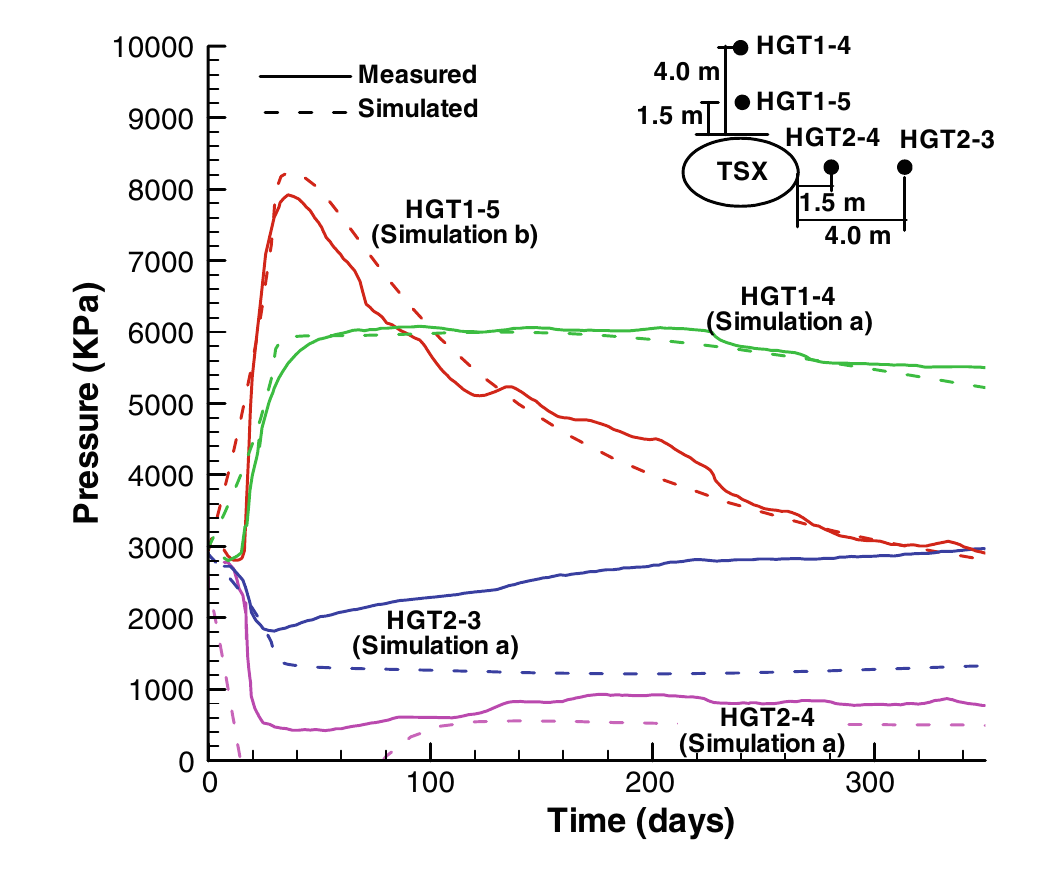
\includegraphics[width=\textwidth]{graphics/TSX_measurement.png}
\caption{Průběh měřeného a simulovaného pórového tlaku v okolí nově vyražené chodby, zdroj \cite{Rutqvist2009}.}
\end{figure}

V rámci projektu DECOVALEX-THMC pak bylo toto měření modelováno čtyřmi týmy s použitím různě složitých hydro-mechanických 
modelů. Na Obr. \ref{fig:TSX} je prezentována velmi dobrá shoda měření a nafitovaného modelu realizovaného týmem LBNL-SKI s využitím kódu ROCMAS. Je použito Mohr-Coulombovo kritérium a empirický vztah 
pro permeabilitu:
\[
   \kappa = \kappa_r + \kappa_{max} \exp(\beta \sigma_m) \exp{\gamma\sigma_d}
\]
kde $\kappa_r,\ \kappa_{max}, \beta, \gamma$ jsou fitované parametry a 
\[
  \sigma_m = \frac{1}{3}(\sigma_1 + \sigma_2 + \sigma_3) - P,
\]
\[
  \sigma_d = \frac{1}{\sqrt{2}}((\sigma_1 - \sigma_2)^2 + (\sigma_2-\sigma_3)^2 + (\sigma_1 - \sigma_3)^2)
\]
jsou střední a deviatorické napětí pro hlavní napětí $\sigma_1,\ \sigma_2,\ \sigma_3$ vypočtené mechanickým modelem.

Bohužel není úplně zřejmé zda bylo použito pouze dat z měření pórového tlaku nebo bylo využito i dalších měření v rámci projektu TSX.
Zdá se však, že další měření zejména výsledky MVP a SEPPI byla použita pouze k počátečním odhadům mechanických a hydraulických parametrů neporušené horniny.


\subsection{Možnosti validace na datech z TSX}
Modely projektu Endorse lze částečně validovat vůči existujícím datům z projektu TSX, 
za předpokladu možnosti jejich získání. 

{\bf Kalibrace modelů.} Po zopakování výše uvedených výsledků lze testvat Bayesovkou inverzi, provést
stochastické výpočty pro zahrnutí vlivu nejistot a ověřit citlivost měření vůči 
parametrům modelu zejména vodivosti v EDZ. 

{\bf Slepá validace.} Vzhledem k velkému množství dalších dat z experimentu TSX lze testovat predikci modelů ENDORSE před ražbou.
V tomto případě by se pro kalibraci modelů (s více škálovým přístupem) využila pouze data o neporušené hornině a 
testovala by se shoda stochastických předpovědí s měřením pórových tlaků. Porovnání s předchozí variantou umožní posoudit 
přínos měření pórového tlaku.


\subsection{Přínosy nového experimentu}
Podobný experiment na PVP Bukov s modifikovaným uspořádáním by pomohl ověřit přínos podobného měření při reálném budování úložiště.

{\bf Anisotropie.} Výše uvedená měření i modely byly realizovány v jednom řezu kolmo na osu díla a není tak možno predikovat anizotropii EDZ s výrazně vyšší vodivostí ve směru paralelním s osou díla. Pro existenci takové anisotropie mluví pozorované uspořádání puklin v EDZ. Pro postižení této anisotropie by bylo nutné realizovat měření ve vrtech umístěných na různých metrážích raženého díla, nebo i těsně před ním. Předchozí modelování by mělo teoreticky ověřit citlivost takového postupu vůči anisotropii permeability.

{\bf Reálné uspořádání.} Měření TSX vyžadovalo sondy ve speciálně situavaných vrtech. V případě realizace podobného experimentu na PVP Bukov lze ověřit
 použitelnost metody i při umístění sond v ukloněných vrtech vedoucích paralelně s osou díla, které je možno realizovat i bez přítomnosti dalších paralelních chodeb. 








\bibliography{zprava.bib}


\pagebreak


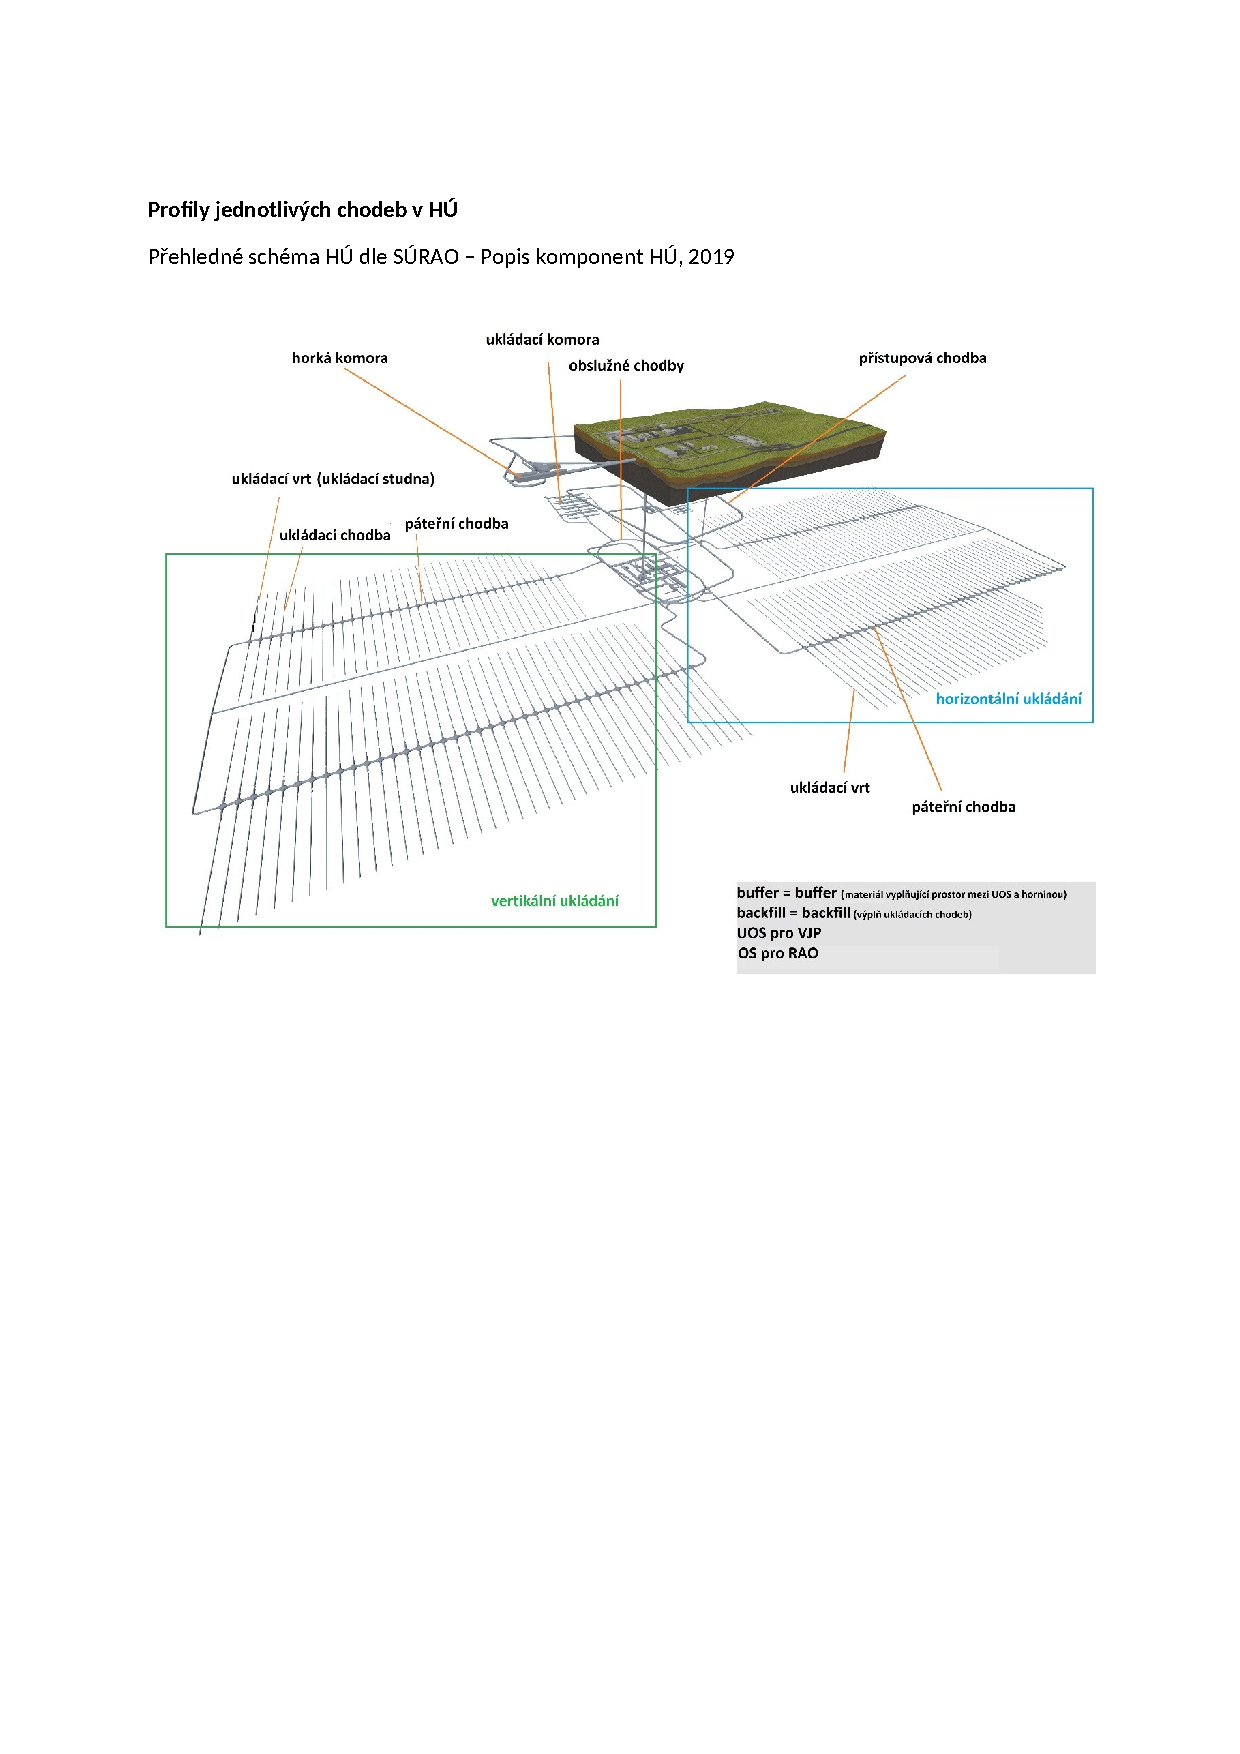
\includepdf[scale=0.99, offset=0 -3cm, page={1},
pagecommand=\section*{Dodatek A - Geometrie HÚ dle SÚRAO}]{Geometrie_HU.pdf}

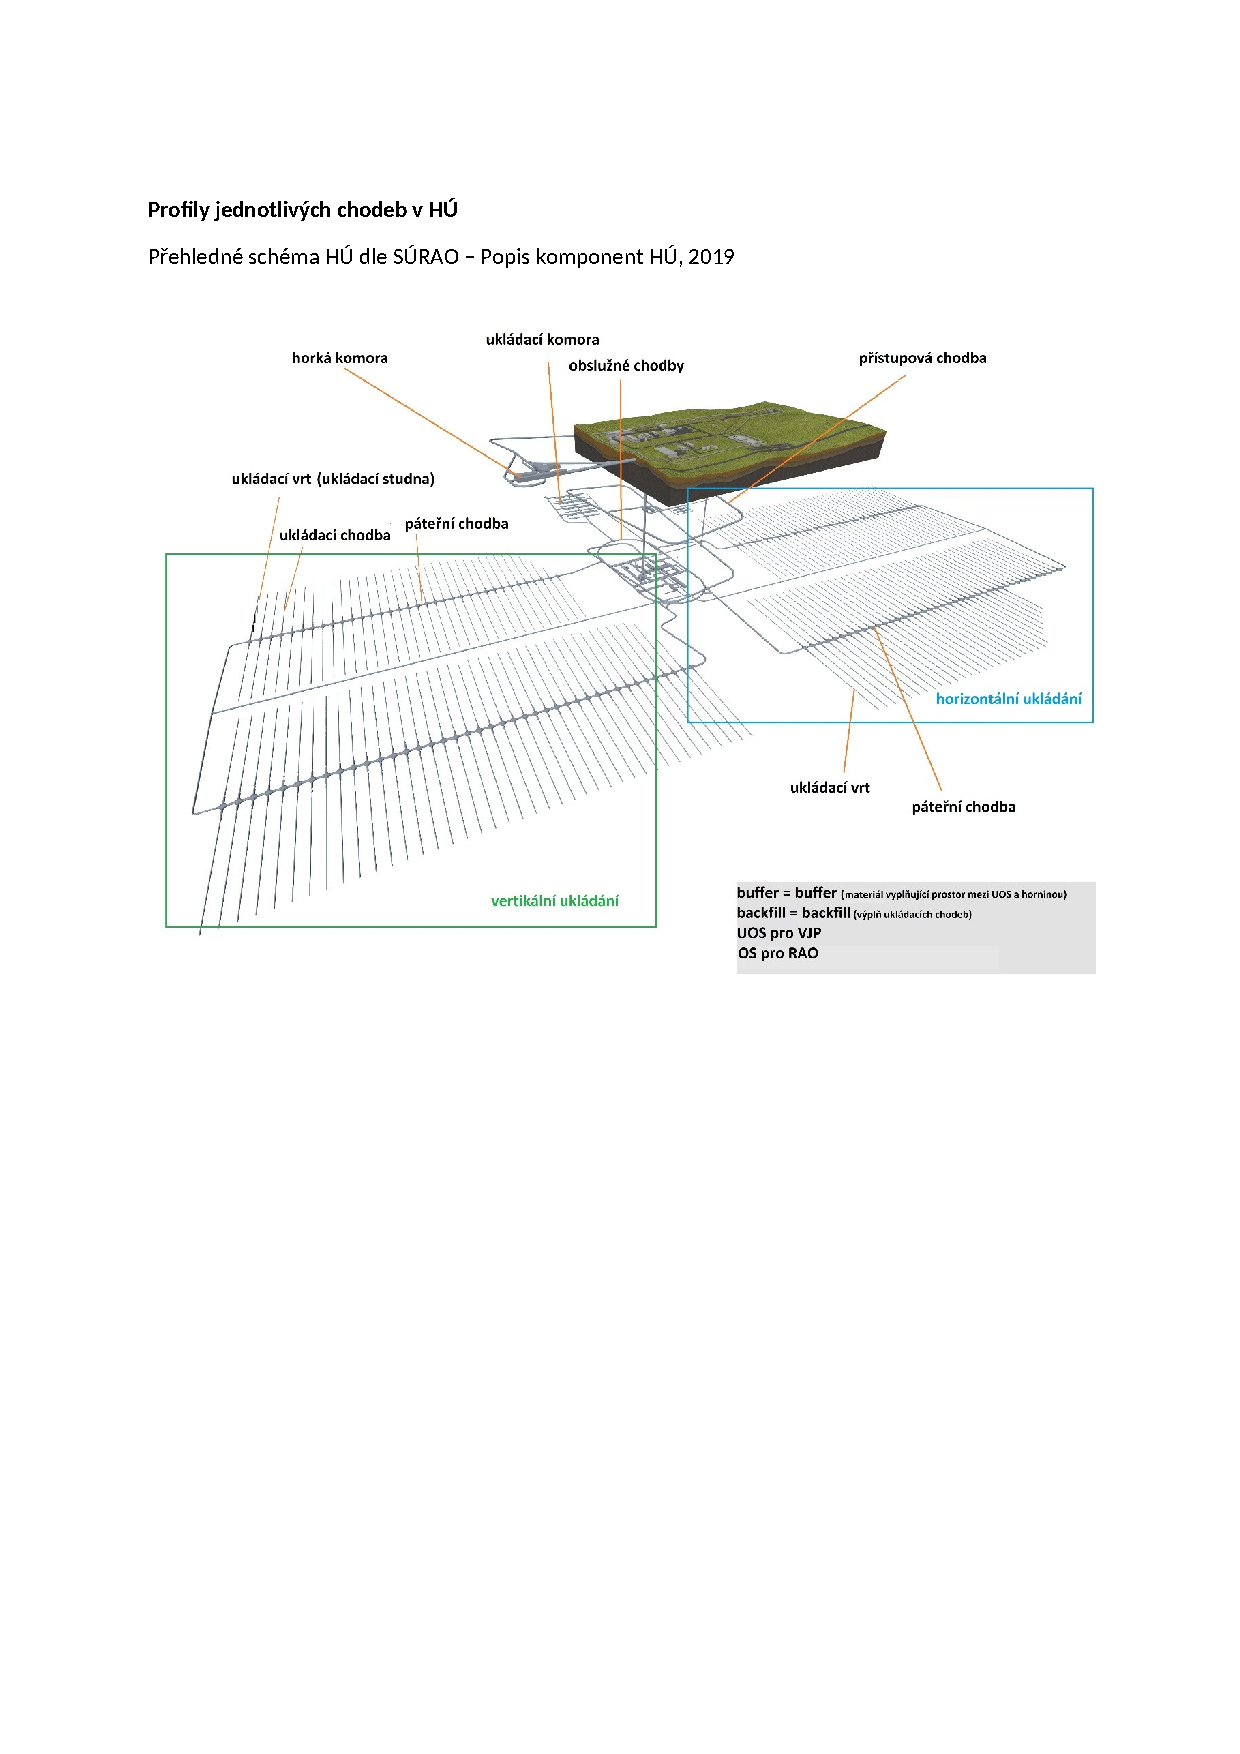
\includepdf[scale=0.99, offset=0 -3cm, page={2,3}]{Geometrie_HU.pdf}

\section*{Dodatek B - odvození řešení rovnice advekce-difúze}
Hledejme nejprve řešení rovnice bez rozpadů na pravé straně:
\begin{equation}
    \label{eq:no_decay_ad}
    R\prtl_t c + v \prtl_x c - d \prtl^2_x c = 0
\end{equation}

pro neznámou koncentraci $c(t, x)$ pro časy $t>0$ a na oblasti $x>0$ s~počáteční podmínkou $c(0, x) = 0$ a
okrajovými podmínkami:
\[
    \prtl_t c(t, \infty) = 0,
\]
\[
    c(t, 0) = c_0(t),
\]
kde $c_0 \in C^\infty$.

Analytická řešení a aproximativní řešení uvedené rovnice pro různé druhy počátečních
a okrajových podmínek lze nalézt v \cite{Genuchten1982} (str. 9). 
Speciálně pro případ skokové okrajové podmínky:
\begin{equation}
    \label{eq:jump_bc}
    c_0(t) = \left\{\begin{array}{ll}
         0 & 0 < t < t_0 \\
         1   & t_0 < t
    \end{array}\right. 
\end{equation}
má rovnice řešení:
\begin{equation}
    \label{eq:jump_sol}
    \tilde c(t, x) = 
    \left\{\begin{array}{ll}
         0                     & 0 < t < t_0 \\
         A(t,x)   & t_0 < t,
    \end{array}\right. 
\end{equation}

kde
\[
    A(t,x) = \frac12 \mathrm{erfc}\Big(\frac{ax-bt}{\sqrt t}\Big)
    + \frac12 e^{cx}\mathrm{erfc}\Big(\frac{ax+bt}{\sqrt t}\Big),
\]
\[
    a = \frac{R}{2\sqrt{dR}},\quad 
    b=\frac{v}{2\sqrt{dR}},\quad 
    c=\frac{v}{d}.
\]

Řešení pro obecný průběh okrajové podmínky $c(t,0) = c_0(t)$ lze napsat v konvolučním tvaru:
\[
    c(t,x) = \int_0^t c_0(s) g(t - s, x) ds,
\]

kde jádro $g(t - s, x)$ je řešením rovnice pro okrajovou podmínku $c_0(t) = \delta(t - s)$. 
Tato okrajová podmínka je formálně derivací jednotkového skoku \eqref{eq:jump_bc}. 
Proto jádro bude derivací odpovídajícího řešení:
\[
    g(t, x) = \prtl_t A(t, x) = 
    \frac{1}{2\sqrt{\pi}} 
    e^{-\big( \frac{ax-bt}{\sqrt{t}}\big)^2}
    \Big[ ax t^{-\frac32} + b t^{-\frac12}\Big]
    + \frac{e^{cx}}{2\sqrt{\pi}}  
    e^{-\big( \frac{ax+bt}{\sqrt{t}}\big)^2}
    \Big[ ax t^{-\frac32} - b t^{-\frac12}\Big].
\]
Tento tvar by měl být použitelný i pro numerický výpočet.


Řešení rovnice s~rozpadovým členem na pravé straně
\[
 R\prtl_t c + v \prtl_x c - d \prtl^2_x c = - \lambda c
\]
pro stejné okrajové a počáteční podmínky pak nalezneme ve tvaru:
\[
    c(t,x) = U(t,x) e^{-\lambda t},
\]
kde $U(t,x)$ řešením rovnice bez rozpadového členu \eqref{eq:no_decay_ad}, ovšem s~okrajovou podmínkou
\[
    \tilde{c}_0(t) = c_0(t) e^{\lambda t}.
\]


% Rovnici vydělíme $R$, označíme
% \[
%     v_r = v/R,\quad d_r = d/R,\quad \lambda_r = \lambda/R.
% \]
% a provedeme transformaci:
% \[
%     c(t, x) = g(t, z),\quad z = \frac{x - v_r t}{\sqrt{d_r}}.
% \]
% Obdržíme rovnici:
% \[
%     \prtl_t g -  \Delta g = - \lambda_r g
% \]
% pro $t>0$, $z > - \frac{v_r t}{\sqrt{d_r}}$, $g(0, z) = 0$, $g(t, \frac{- v_r t}{\sqrt{d_r}}) = c_0(t)$.

% Její řešení má tvar:
% \[
%   g(t,z) = G(t,z) e^{-\lambda_r t}
% \]
% kde $G(t, z)$ je řešení homogenní rovnice:
% \[
%     \prtl_t G -  \Delta G = 0
% \]
% s okrajovou podmínkou $G(t, \frac{- v_r t}{d_r}) = c_0(t) e^{\lambda_r t}$.

% Jádro $\phi(t, z)$ pro 


% \begin{equation}
%     g(t, z) = (4\pi t)^{-\frac12} e^{\frac{-z^2}{4t}} e^{-\lambda_r t},\quad
%     ,
% \end{equation}
% kde jsme označili




\end{document}
